%%%%%%%%%%%%%%%%%%%%%%%%%%%%%%%%%%%%%%%%%%%%%%%%%%%%%%%%%%%%%%%%%%%%%%
% LaTeX Vorlage: Mathematische Texte
%
% Quelle: http://www.mi.uni-koeln.de/wp-MIEDV/% Datum: Juli 201% Copyright Universität zu Köln
% 
%%%%%%%%%%%%%%%%%%%%%%%%%%%%%%%%%%%%%%%%%%%%%%%%%%%%%%%%%%%%%%%%%%%%%%
\documentclass[12pt,a4paper,twoside, open=right]{scrreprt}

\addtokomafont{sectioning}{\rmfamily}
%\usepackage[ngerman]{babel}% deutsches Sprachpaket wird geladen
\usepackage[ngerman,english]{babel}% englisches Sprachpaket wird geladen
\usepackage{tabularx}
%\usepackage{lmodern}% Für die Schrift
\usepackage[T1]{fontenc} % westeuropäische Codierung wird verlangt
\usepackage[utf8]{inputenc}% Umlaute werden erlaubt
\usepackage[usenames]{color} % Erlaubt die Benutzung der namen im Farbpaket und deren Änderung
%\usepackage{showkeys} % Labels anzeigen
\usepackage{amsmath} % Erweiterung für den Mathe-Satz
\usepackage{amssymb} % alle Zeichen aus msam und msmb werden dargestellt
\usepackage{framed}
\usepackage[german]{fancyref}
\usepackage{listings}
\usepackage{color}
\definecolor{mygreen}{RGB}{28,172,0} % Define colour
\definecolor{mylilas}{RGB}{170,55,241}
\usepackage{graphicx} % Graphiken und Bilder können eingebunden werden
\usepackage{multirow} % erlaubt in einer Spalte einer Tabelle die Felder in mehreren Zeilen zusammenzufassen
\usepackage{enumerate} % erlaubt Nummerierungen 
\usepackage{url} % Dient zur Auszeichnung von URLs; setzt die Adresse in Schreibmaschinenschrift.
\usepackage[center]{caption}  % Bildunterschrift wird zentriert
\usepackage{subfigure} % mehrere Bilder können in einer figure-Umgebung verwendet werden
\usepackage{longtable} % Diese Umgebung ist ähnlich definiert wie die tabular-Umgebung, erlaubt jedoch mehrseitige Tabellen.
\usepackage{paralist} % Modifikation der bereits bestehenden Listenumgebungen
\usepackage{amsthm} % erlaubt die Benutzung von eigenen Theoremen
\usepackage{hyperref} % Links und Verweise werden innerhalb von PDF Dokumenten erzeugt
\usepackage{wrapfig} % Das Paket ermöglicht es von Schrift umflossene Bilder und Tabellen einzufügen.
%\numberwithin{equation}{section} % Nummerierungen der Gleichungen, die durch equation erstellt werden, sind gebunden an die section
\usepackage{latexsym} % LaTeX-Symbole werden geladen
\usepackage{tikz} % Erlaubt es mit tikz zu zeichnen
\usepackage{tabularx} % Erlaubt Tabellen 
\usepackage{algorithm} % Erlaubt Pseudocode
\usepackage{algorithmic}
\usepackage{color} % Farbpaket wird geladen
\usepackage{stmaryrd} % St Mary Road Symbole werden geladen
\usepackage{csquotes}
\usepackage{bm}
\usepackage{todonotes}
\usepackage{lipsum}
\usepackage{multicol}

% Hier werden neue Theorems erstellt.
\theoremstyle{definition}
\newtheorem{auf}{Aufgabe}
\newtheorem{rem}[auf]{Remark}
\newtheorem{defn}[auf]{Definition}
\newtheorem{bsp}[auf]{Example}
\newtheorem{notation}[auf]{Notation}
\theoremstyle{plain}
\newtheorem{kor}[auf]{Corollary}
\newtheorem{sa}[auf]{Theorem}
\newtheorem{lem}[auf]{Lemma}
\newtheorem{alg}[auf]{Algorithm}
\DeclareMathOperator*{\esssup}{ess\,sup} % essentiellen Supremums
\DeclareMathOperator{\spn}{span} % Span
\DeclareMathOperator{\supp}{supp} % Träger
\DeclareMathOperator{\ddiv}{div} % divergenz
\newcommand{\abs}[1]{\left\vert #1\right\vert}
\newcommand{\dotp}[2]{\left\langle #1,#2\right\rangle}
\newcommand{\rr}{\mathbb{R}}
\newcommand{\g}{~\textgreater ~}
\newcommand{\ls}{~\textless ~}
\renewcommand{\algorithmicrequire}{\textbf{Input:}}
\renewcommand{\algorithmicensure}{\textbf{Output:}}
\newcommand{\cc}{\mathbb{C}}
\newcommand{\kk}{\mathbb{K}}
\newcommand{\nn}{\mathbb{N}}
\newcommand{\qq}{\mathbb{Q}}
\newcommand{\e}{\varepsilon\g 0~}
\newcommand{\fe}{\forall \e}
\newcommand{\so}{\sum_{k=0}^{n}}
\newcommand{\si}{\sum_{k=1}^{n}}
\newcommand{\soi}{\sum_{k=0}^{\infty}}
\newcommand{\sii}{\sum_{k=1}^{\infty}}
\newcommand{\de}{\mathrm{d}}
\newcommand{\norm}[1]{\left\lVert#1\right\rVert}
\newcommand{\lpnorm}[1]{\left(\int\abs{#1}^2\D\Omega \right)^{1/2}}
\newcommand{\ltnorm}[1]{\norm{#1}_{\mathrm{L}^2}}
\newcommand{\bfu}{\bm{u}}
\newcommand{\bff}{\bm{f}}
\newcommand{\bfB}{\bm{B}}
\newcommand{\bfb}{\bm{b}}
\newcommand{\bfs}{\bm{s}}
\newcommand{\bfC}{\bm{C}}
\newcommand{\bfx}{\bm{x}}
\newcommand{\bfR}{\bm{R}}
\newcommand{\tpne}{\tilde\phi_{n+1}}
\newcommand{\tpn}{\tilde\phi_{n}}
\newcommand{\D}{\mathop{}\!\mathrm{d}}
\floatname{algorithm}{Algorithmus}
\renewcommand{\thesubfigure}{\thefigure.\arabic{subfigure}}
\addto{\captionsenglish}{\renewcommand{\bibname}{References}}
\lstset{language=Matlab,
    basicstyle={\scriptsize \ttfamily},
    breaklines=true,
    morekeywords={matlab2tikz},
    keywordstyle=\color{blue},
    morekeywords=[2]{1}, 
    keywordstyle=[2]{\color{black}},
    identifierstyle=\color{black},
    stringstyle=\color{mylilas},
    commentstyle=\color{mygreen},
    showstringspaces=false, %without this there will be a symbol in the places where there is a space
    numbers=left,
    numberstyle={\tiny \color{black}}, % size of the numbers
    numbersep=9pt, % this defines how far the numbers are from the text
    emph=[1]{for,end,break},
    emphstyle=[1]\color{red}, %some words to emphasise
}
\makeatletter
\renewcommand{\p@subfigure}{}
\renewcommand{\@thesubfigure}{\thesubfigure:\hskip\subfiglabelskip}
\makeatother
\begin{document}
% Hier wird die Titelseite erstellt
\begin{titlepage}
\pagestyle{empty}
\begin{center}
\newcommand{\HRule}{\rule{\linewidth}{0.7mm}}
\textsc{\LARGE University of Cologne }\\ [0.4cm]
\textsc{ Department of Mathematics} \\[1.5cm]

\includegraphics[width=0.45\textwidth]{uni}\\[1.5cm]  % Uni-Logo wird geladen
\HRule \\[0.4cm]
{ \huge \bfseries Numerical Solution of Integro-Differential equations}\\[0.4cm]
\HRule \\[1cm]
\textsc{\Large Master's thesis}\\[2mm]
\textsc{\today}\\[10mm]
\textsc{in cooperation with the German Aerospace Center}\\[1.0cm]

\includegraphics[width=0.45\textwidth]{DLR-Logo-full}\\[1.0cm]


  




\begin{center}

\textsc{\Large Nils Dornbusch} \\[3pt]
\textsc{\Large first examiner: Prof. Dr-Ing. Gassner}
\end{center}
\end{center}
\end{titlepage}
\begin{otherlanguage}{ngerman}
  

\chapter*{Danksagung}
\lipsum[1]
%Ich möchte mich bei Herrn Professor Gassner und seiner Arbeitsgruppe ganz herzlich für die kompetente und umfangreiche Betreuung bedanken. Insbesondere bei Herrn Lucas Friedrich für sein außerordentliches Engagement, das weit über Sprechstundenzeiten hinaus ging. 
%\par Zusätzlich bedanke ich mich noch bei meiner Familie, meinen Freunden und Kommilitonen und meiner Freundin für ihre Geduld und ihr Verständnis.
%\\[1cm]
Köln, \today 
\\[1cm]
Nils Dornbusch
\end{otherlanguage}
\newpage
\tableofcontents
\newpage
\chapter{Introduction}
\lipsum[1]
%This work aims to provides an analysis of the Integro-Differential-equations which occur when modeling the behaviour of non-Newtonian fluids. The motivation arises in Physics when studying for example liquid glass or granule. This is often needed in space applications. I will reference the relevant physical phenomena which the interested reader can follow to learn more about as this is not the main focus of this work.\\
%The main focus will actually lie in the numerical challenges, which the equations present. We will also touch upon issues regarding the implementation.
%\par 
%The biggest problem when trying to implement these equation lies in the Integral over older timesteps and the appearence of another time dimension, which we call the \enquote{age dimension}. But more on that later on.\\
%We will take the following steps to study said equations:
%\begin{itemize}
%    \item theoretical derivation of the Navier-Stokes-Equations for the non-Newtonian stress tensor
%    \item discussion of different spatial and time discretization methods
%    \item challenges in the implementation
%    \item some application with different complexity 
%\end{itemize}
%For the sake of simplicity we will use the well known framework FEniCS \cite{Alnaes2012a}\cite{AlnaesBlechta2015a}\cite{AlnaesEtAl2012}\cite{AlnaesLoggEtAl2012a} which uses the underlying DOLFIN library \footnote{citation needed} and we will make assumptions that reduce the complexity of the problem. \par 
%At the end of this work we would like to answer the question: \enquote{Is this numerical method worth to try with the full system in 5-dimensions (3 spatial + 1 time  + 1 age dimension) in exa-scale systems?}\par 
%So without further ado let us dive into the matter!
\newpage
\chapter{Mathematical basics}
In this chapter, various definitions and theorems are presented, which will be used extensively throughout this work. Most of them are just a recap of well known theorems and are therefore presented without proof. The interested reader may follow the literature referenced in each section.
\section{Basics and notation}
In the beginning, we will quickly state basic mathematical facts and introduce some notation, which we will use throughout this work. Most of this should be self explanatory.
\begin{notation}
    We will use $\nn$ as the natural numbers starting from 1, and $\rr,\cc,\qq$ denote the real, complex and rational numbers. With $\kk$ we denote a field, which can be $\rr$ or $\cc$. $\nn_0$ represent the natural numbers starting from 0. $\rr^+_0$ shall denote $[0,\infty)$.
\end{notation} 
\section{Functional analysis}
\label{sec:funcana}
Here, we cover basics of functional analysis as necessary for this work and the finite element method especially. We will follow \cite{Ganesan2017} for this.
\begin{defn}[Norm]
    Let $X$ be a $\kk$ vector space. A mapping $\norm{\cdot}\colon X\to\rr$ is called a \emph{norm} on $X$ if 
    \begin{align}
        1. &\norm{x}=0 \Leftrightarrow x=0 &&\forall x\in X  &&\text{(positive definite)},\\
        2. &\norm{\lambda x}=\abs{\lambda}\norm{x} &&\forall x\in X,\lambda\in\kk &&\text{(homogeneous)},\\
        3. &\norm{x+y}\le\norm{x}+\norm{y}&&\forall x,y\in X &&\text{(triangle inequality)}.
    \end{align}

    We call the pair $(X,\norm{\cdot})$ a \emph{normed space}.
\end{defn}
\begin{rem}
    It follows directly from the definition that $\norm{x}\ge 0 \quad\forall x\in X$.
\end{rem}
\begin{defn}[\textsc{Cauchy} sequence]
    A sequence $(x_n)_{n\in\nn}$ is called \emph{\textsc{Cauchy} sequence} if
    \begin{equation}
         \forall\varepsilon>0 \exists n_0(\varepsilon)\in\nn\colon \forall m,n>n_0\text{ it holds that }\norm{x_m-x_n}<\varepsilon.
    \end{equation}
\end{defn}
\begin{defn}[Convergence]
    A sequence $(x_n)_{n\in\nn}$ converges to $x\in X$ if 
    \begin{equation}
        \forall\varepsilon>0 \exists n_0(\varepsilon)\colon \forall n>n_0 \text{ it holds that } \norm{x_n -x}<\varepsilon.
    \end{equation}
\end{defn}
As one might know, a \textsc{Cauchy} sequence does not converge in general. The class of spaces, for which this is true, is given in the following definition.
\begin{defn}
    A normed space $(X, \norm{\cdot})$ is called \emph{complete} if every \textsc{Cauchy} sequence in $X$ converges in $X$. A complete normed space is also called a \textsc{Banach} \emph{space}.
\end{defn}
From now on let $\Omega$ be an open and bounded subset of $\rr^n$.
\begin{defn}
    For a function $f\colon\Omega\to\rr$ we define the norm
     \begin{equation}
    \norm{f}_{p}:=\left(\int_\Omega\abs{f}^p\D\Omega\right)^{1/p}
    \end{equation}
    and
     \begin{equation}
    \norm{f}_{\infty}:=\esssup\{\abs{f(x)}\colon x\in\Omega\}.
    \end{equation}
    However, this is only a norm if we identify functions, which only differ on sets of zero measure. As usual the sets of equivalence classes of almost everywhere identical functions for which $\norm{f}_p<\infty$ is denoted by $\mathrm{L}^p(\Omega)$.
\end{defn}
\begin{lem}[\textsc{Minkowski}'s inequality]
    For $f,g\in L^p(\Omega)$ and $p\in[1,\infty]$, we have
    \begin{equation}
        \norm{f+g}_p\le\norm{f}_p+\norm{g}_p
    \end{equation}
\end{lem}
\begin{sa}
    The space $L^p(\Omega)$, $p\in[1,\infty]$ is a \textsc{Banach} space.
\end{sa}
\begin{defn}
    Let $V$ be a $\kk$ vector space. A mapping $\dotp{\cdot}{\cdot}\colon V\times V\to\rr$ is called an \emph{inner product} or \emph{dot product} if 
    \begin{enumerate}
        \item $\dotp{u}{u} \ge 0 \quad \forall u\in V$ (positive definite),
        \item $\dotp{u}{u} = 0 \Leftrightarrow u=0 $  (strictly positive),
        \item $\dotp{u}{v} = \overline{\dotp{v}{u}}   \quad\forall u,v\in V$ (conjugate symmetric),
        \item $\dotp{u}{\lambda v} = \lambda\dotp{u}{v} \quad\forall u,v\in V,\lambda\in\kk$ (homogeneous in second argument),
        \item $\dotp{u}{v+w} =\dotp{u}{v}+\dotp{u}{w} \quad\forall u,v\in V$ (linear in second argument).
    \end{enumerate}
\end{defn}
\begin{rem}
    In the case that $V$ is a real-valued vector space, the inner product is trivially linear and homogeneous in the first argument. Even in the complex case, we get these properties, but with conjugation.
\end{rem}
\begin{sa}
    Let $V$ be a vector space and $\dotp{\cdot}{\cdot}$ an inner product. By setting $\norm{v}_V:=\sqrt{\dotp{v}{v}}$, we obtain a norm. Thus every vector space with an inner product is a normed space.
\end{sa}
\begin{defn}
    A complete vector space with an inner product is called a \emph{\textsc{Hilbert} space}.
\end{defn}
\begin{sa}[\textsc{Cauchy-Schwarz} inequality]
    \label{sa:Schwarz}
    Let $V$ be a vector space. Then 
    \begin{equation}
        \abs{\dotp{u}{v}}\le\norm{u}_V\norm{v}_V\quad \forall u,v\in V.
    \end{equation}
\end{sa}
\begin{sa}[\textsc{Hölder's} inequality]
    \label{sa:hoelder}
    Let $f,g \colon V\to\kk$ be functions with the necessary regularity and $\frac{1}{p}+\frac{1}{q}=1$. It holds
    \begin{equation}
        \int\abs{fg}\D V\le\left(\int\abs{f}^p\D V\right)^{1/p}\left(\int\abs{g}^q\D V\right)^{1/q}
    \end{equation}
\end{sa}
\begin{bsp}
    $V=\mathrm{L}^2(\Omega)$ with the inner product
    \begin{equation}
       \dotp{f}{g}:=\int_\Omega f(x)g(x)\D x
    \end{equation}
    is a \textsc{Hilbert} space.
\end{bsp}
\begin{notation}
    We write $\mathrm{C}^k(\Omega)$, $k\in\nn\cup\{\infty\}$ for the space of $k$ times differentiable functions on $\Omega$. $\mathrm{C}^0(\Omega)$ shall be the space of continuous functions on $\Omega$.
\end{notation}
\begin{defn}
    The \emph{support} of a function $f\colon \Omega\to\rr$ is defined by 
    \begin{equation}
        \supp f = \overline{\{x\in\Omega\colon f(x)\neq 0\}}.
    \end{equation}
\end{defn}
\begin{notation}
    In the following sections and chapters we will often use functions with compact support, so we will introduce the convention
    \begin{equation}
        \mathrm{C}^k_0(\Omega)=\{f\in \mathrm{C}^k(\Omega)\colon \supp f \text{ is compact} \},
    \end{equation}
    where we mean \enquote{compact} in the topological sense, so in our cases bounded and closed.
\end{notation}
\begin{rem}
    Interestingly, one can proof that if $f\in \mathrm{C}^k_0$, then $f$ approaches zero on the boundary $\partial\Omega$. This motivates the notation.
\end{rem}
\begin{defn}
    We define 
    \begin{equation}
        \mathrm{L}^1_{\mathrm{loc}}(\Omega):=\{f\colon\Omega\to\rr\colon f\in \mathrm{L}^1(A) \text{ for all compact} A\subset\Omega \},
    \end{equation}
    as the space of \emph{locally integrable functions}.
\end{defn}
\begin{bsp}
    $\mathrm{L}^1_\mathrm{loc}$ is a true extension of $\mathrm{L}^1$. Consider $f(x)=\frac{1}{x}$ on $(-1,1)$. $f$ belongs to $\mathrm{L}^1_\mathrm{loc}(-1,1)$, but not to $\mathrm{L}^1(-1,1)$. 
\end{bsp}
\begin{defn}
    \label{defn:weakderivative}
    Let $\alpha\in\nn^n_0$ be a multi index. A function $f\in \mathrm{L}^1_{loc}(\Omega)$ has a \emph{weak derivative} $\nu=D^\alpha f\in \mathrm{L}^1_\mathrm{loc}(\Omega)$ if $\forall \varphi\in \mathrm{C}_0^\infty$
    \begin{equation}
        \int_\Omega\nu\varphi\D\Omega = (-1)^{\abs{\alpha}}\int_\Omega fD^\alpha\varphi \D\Omega,
    \end{equation}
    where 
    \begin{equation}
        D^\alpha\varphi=\frac{\partial^{\abs{\alpha}}\varphi}{\partial x_1^{\alpha_1}\dotsb\partial x_n^{\alpha_n}}.
    \end{equation}
\end{defn}
\begin{rem}
    This definition is motivated by the integration by parts method. One wants to find functions that obey integration by parts but are not necessarily differentiable in the classical sense. However, if $f$ is differentiable then the weak and classic derivatives match. IT is also important to note that the weak derivative of a function, if it exists, is unique if we identify functions, which only differ on sets of zero measure.
\end{rem}
\begin{defn}
    We denote by $W^{m,p}(\Omega)$, for $p\in[1,\infty]$ and $m\ge 0$, the set of all functions $f\in \mathrm{L}^p(\Omega)$ with weak derivatives in $\mathrm{L}^p(\Omega)$ up to the order $\abs{\alpha}\le m$. These sets are called \textsc{Sobolev} \emph{spaces}. We denote $\mathrm{H}^m(\Omega):=W^{m,2}(\Omega)$ because these are special, as one can see in the following theorem.
\end{defn}
\begin{sa}
    The \textsc{Sobolev} space $W^{m,p}(\Omega)$ with the norm
    \begin{equation}
        \norm{f}_{W^{m,p}}:=\left(\int_\Omega\sum_{\abs{\alpha}\le m}\abs{D^{\alpha} f(x)}^p\D\Omega\right)^{1/p},
    \end{equation}
    for $p\in[1,\infty)$, and 
    \begin{equation}
        \norm{f}_{W^{m,p}}:=\max_{\abs{\alpha}\le m}\left(\esssup_{x\in\Omega}\abs{D^{\alpha}f(x)}\right)
    \end{equation}
    if $p=\infty$, is a \textsc{Banach} space. $\mathrm{H}^m(\Omega)$ with the inner product
    \begin{equation}
        \dotp{u}{v}_{\mathrm{H}^m}:=\sum_{\abs{\alpha}\le m}\dotp{D^{\alpha}u}{D^{\alpha}v}=\sum_{\abs{\alpha}\le m}\int_\Omega D^\alpha u D^\alpha v\D\Omega \quad \forall u,v\in \mathrm{H}^m(\Omega)
    \end{equation}
    is a \textsc{Hilbert} space.
\end{sa}
\begin{rem}
    The $\mathrm{H}^m$ spaces are very important for all numerical methods because of their property that they are \textsc{Hilbert} spaces. The whole theory, which follows hereafter, relies heavily on this assumption.
\end{rem}

\section{The finite element method}
\label{sec:fem}
This section covers the basics of the finite element method (FEM). This is a standard approach, which is used in almost every book about this topic. We still use \cite{Ganesan2017} as a reference.
Let us start by introducing the concept of \emph{weak solutions}. Consider the \textsc{Poisson} problem
\begin{equation}
    -\Delta u = f \quad \text{in }\Omega
\end{equation}
and $u=0$ on the boundary, where $u,f\colon \Omega\to\rr$. This formulation requires $u\in \mathrm{C}^2(\Omega)$ for $f\in\mathrm{C}^0(\Omega)$, which is a very strong assumption. In other examples this often excludes the physical solution, so we want to reduce the required regularity. For this, we integrate both sides over $\Omega$ and multiply with a testfunction $\varphi\in \mathrm{C}^\infty_0(\Omega)$. So we get
\begin{equation}
    -\int_\Omega \Delta u\varphi\D\Omega =\int_\Omega f\varphi\D\Omega.
\end{equation}
If we now use \textsc{Green}'s theorem on the left side, we get
\begin{equation}
    \int_\Omega \nabla u\cdot\nabla \varphi\D\Omega = \int_\Omega f\varphi\D\Omega \quad\forall\varphi\in \mathrm{C}^\infty_0(\Omega)\label{eq:laplace}.
\end{equation}
We call this equation the \emph{weak formulation}.
The boundary term has vanished because $\varphi$ is assumed to be 0 on the boundary.
We can observe that we can use \textsc{Green} here because we assume $u\in \mathrm{C}^2(\Omega)$. But this equations imposes much fewer regularity requirements then the classical formulation. We only need $u\in\mathrm{H}^1(\Omega)$ to satisfy the equation. The space of acceptable solutions is now more extensive than before.

\begin{defn}
    Let $V$ be a \textsc{Hilbert} space. A bilinear form (e.g. inner product) $a\colon V\times V\to\rr$ is said to be \emph{continuous} if there exists a constant $\beta>0$ such that
    \begin{equation}
        \abs{a(u,v)}\le\beta\norm{u}\norm{v}\quad \forall u,v\in V,
    \end{equation}
    and \emph{coercive} if 
    \begin{equation}
        \exists\alpha>0\colon \quad a(u,u)\ge \alpha\norm{u}^2\quad\forall u\in V.
    \end{equation}
\end{defn}
\begin{rem}
    We see that if $a$ is the inner product of $V$ and induces the norm, then both properties are satisfied. The first identity is simply the \textsc{Schwarz} inequality and the second is fulfilled by definition. In this case $\sqrt{a(v,v)}$ is called \emph{energy norm}, which is the natural norm for error analysis of this problem.
\end{rem}
\begin{sa}[\textsc{Lax-Milgram}]
    \label{sa:LaxMilgram}
    Let $V$ be a \textsc{Hilbert} space, $a(\cdot,\cdot)$ be a continuous coercive bilinear form and $F$ a continuous linear functional. Then there exists a unique $u\in V$ such that
    \begin{equation}
        a(u,v)=F(v)\quad \forall v\in V.
    \end{equation}
\end{sa}
\begin{rem}
    Why is this relevant to us? On first glance it is not obvious what this has to do with numerical approximations. It turns out that any linear partial differential equation (linear PDE) in weak formulation can be written in this form, where $u$ are the unknowns and $v$ is a testfunction.
\end{rem}
\begin{bsp}
    Let us revisit \eqref{eq:laplace}. We can see that we can rewrite it in terms of $a$ and $F$. 
    \begin{equation}
        a(u,v):=\int_\Omega \nabla u\cdot \nabla v\D\Omega
    \end{equation}
    and $F=\int f\D\Omega$ remains the same. Note, that $a$ is not an inner product in the strict sense on $\mathrm{H}^1(\Omega)$ here. Consider $u\equiv c$ for $c\in\rr$ constant. Then $a(u,u)=0$ but $u$ is not necessarily zero. So we get a so called \emph{seminorm} if we use $p(u):=\sqrt{a(u,u)}$. All properties are the same, as a normal norm would have, but the zero uniqueness. However, on $\mathrm{H}^1_0(\Omega)$ this is an inner product so we can still deduce that this problem has a unique solution for a given set of boundary conditions.
\end{bsp}
\subsection{Standard \textsc{Galerkin} method}
So far we only covered the theory behind PDEs. We know in which space our solution lives, and we can now try all linear combinations for a given basis and are finished. Unfortunately it is not that easy. Recall that $u\in \mathrm{H}^1_0(\Omega)$ in our example earlier. The problem is that $\mathrm{H}^1(\Omega)$ is a space of infinite dimension. Because no computer can handle infinitly many cases, we have to reduce the problem somehow. Thus we use finite dimensional subspaces of the solution space and calculate the best approximation in this subspace. How this spaces are constructed exactly, will be explained later on. 
\par 
Let $V$ a \textsc{Hilbert} space and our solution space. Furthermore let $V_h\subset V$ be an $n\in\nn$ dimensional subspace with a discretization parameter $h$. We want that our discrete solution converges to the continuous one, when $h\to 0$. Because the properties of $a$ and $F$ are also fulfilled in $V_h$, the \textsc{Lax-Milgram} theorem still guarantees existence and uniqueness of the solution. Our new problem is given by
\begin{equation}
    a(u_h,v_h) = F(v_h) \quad \forall v_h\in V_h \label{eq:galerkindiscrete}
\end{equation}
for the discrete solution $u_h\in V_h$.
We will rewrite \eqref{eq:galerkindiscrete} as a linear system of equations. By $\{\varphi_i\}$ for $i=1,\dotsc,n$, we denote a basis of $V_h$. Obviously, there exist coefficients $(U_j)_1^n\subset\rr$ so that
\begin{equation}
    u_h(x)=\sum_{j=1}^{n}U_j\varphi_j(x),\quad \nabla u_h(x)=\sum_{j=1}^{n}U_j\nabla\varphi_j(x).
\end{equation}
The coefficients $U_j$ are also called degrees of freedom or unknowns. Because we have a basis for $V_h$, we can rewrite \eqref{eq:galerkindiscrete} as 
\begin{equation}
    a\left(\sum_{j=1}^{n}U_j\varphi_j(x),\varphi_i\right)= F(\varphi_i)\quad \forall i=1,\dotsc,n.
\end{equation}
If we recall that $a$ is a bilinear form, we can also write
\begin{equation}
    \sum_{j=1}^{n}U_ja(\varphi_j,\varphi_i)=F(\varphi_i) \quad\forall i=1,\dotsc,n.
\end{equation}
This already looks like a matrix vector multiplication. So let us define $a_{i,j}=a(\varphi_j,\varphi_i)$ and $b_i=F(\varphi_i)$. We get the following linear problem
\begin{equation}
    AU=b,
\end{equation} which can be solved by any of the many known linear solvers. The matrix $A$ is often called \emph{stiffness matrix} and $b$ the \emph{load vector}.
\begin{rem}
    What happens if the problem is not linear? One would then still use a weak formulation. This would then be interpreted as a problem of the form
    \begin{equation}
        F(u,v) = 0 \quad\forall v \in V.
    \end{equation}
    This would then be treated with basis functions of $V_h$ as above, but one would have to take care choosing a right basis $\varphi$. It can then be rewritten as 
    \begin{equation}
        F(u_h, \varphi_i) = 0 \quad \forall i=1,\dotsc,n.
    \end{equation}
    This would then be plugged into a non-linear solver. However, existence or even uniqueness cannot be guaranteed and must be assessed on a case-by-case basis. This is an open research topic.
\end{rem}
\subsection{Finite element spaces}
For now, we handled the problem with an arbitrary subspace $V_h$. But how would we choose such space and its basis functions?
\begin{notation}
    We denote by
    \begin{equation}
        P_k(K):=\left\{p\colon K\to\rr\left\vert p(x)=\sum_{\abs{\alpha}\le k}c_ax^a,\right.\quad x\in K\right\}
    \end{equation}
    the set of all polynomials of degree less than or equal to $k$. $c_a$ are constant coefficients.
\end{notation}
We will construct a mesh by starting with a decomposition $\tau_h$ of $\Omega$ into open cells $K$ with $\overline{\Omega}=\bigcup_{K\in\tau_h}\overline{K}$.
\begin{defn}
    We use $\Sigma_k$ as the set of degrees of freedom. These are given as linear nodal functionals $N_i(v)$ for $i=0,\dotsc,n$, where $n= \dim P_k -1$. $(K,P_k,\tau_h)$ is called a \emph{finite element}. If $N_i(v)$ is given by $N_i(v)=v(a_i)$, where $a_i$ is a set of points, we call $(K,P_k,\tau_h)$ a \textsc{Lagrange} \emph{finite element}. The points $a_i$ are called \emph{nodes} of the finite element.
\end{defn}

    We defined finite elements, but not all $\tau_h$ are admissible.
\begin{defn}
    A decomposition of the domain $\Omega\subset\rr^d$ into cells $K\in\tau_h$ is admissible if
    \begin{enumerate}
        \item $\overline{\Omega}=\bigcup_{K\in\tau_h}\overline{K}$,
        \item any nonempty intersection of two cells $\overline{K_1}\cap\overline{K_2}$ is either a vertex, an edge or a face of both cells.
    \end{enumerate}
\end{defn}
How do we construct $V_h$ from here so that $V_h\subset \mathrm{H}^1(\Omega)$?
\begin{defn}
    For $v_h\in V_h$ we want that $v_h\vert_K\in P_k$. This requirement is enough to define $v_h\vert_K$ uniquely because for each $x\in K$ the degrees of freedoms are linear independent.
\end{defn}
The following theorem ensures us that the combination of all cells still results in $V_h$ being a subset of $\mathrm{H}^1(\Omega)$.
\begin{sa}
    If for every $K\in\tau_h,P_k\subset \mathrm{H}^1(K)$, and $V_h\subset \mathrm{C}^0(\Omega)$, then $V_h\subset \mathrm{H}^1(\Omega)$.
\end{sa}
Because this may not be a well known theorem, we will give a proof here.
\begin{proof}
    Let $v\in V_h$ be given. If we can show that the weak derivatives $D^\alpha v\in \mathrm{L}^2(\Omega)$ for $\abs{\alpha}=1$. The natural choice would be the piecewise defined function $w:=D^\alpha(v\vert_K)\in \mathrm{L}^2(K)$. Let $\varphi\in \mathrm{C}^\infty_0(\Omega)$ be arbitrary. It holds that 
    \begin{equation}
        \int_\Omega(w\varphi+vD^\alpha \varphi)\D x = \sum_{K\in\tau_h}\int_K(D^\alpha(v\vert_K)\varphi+v\vert_K D^\alpha\varphi)\D x,
    \end{equation}
    where we just used the linearity of the integral. If we recall the definition of the weak derivative (definition \ref{defn:weakderivative}), we can see how we can rewrite $D^\alpha(v\vert_k)$. We obtain
    \begin{align}
        \sum_{K\in\tau_h}\int_K(D^\alpha(v\vert_K)\varphi+v\vert_K D^\alpha\varphi)\D x&=\sum_{K\in\tau_h}\left(-\int_K v\vert_KD^\alpha\varphi+\int_K v\vert_K D^\alpha\varphi +\int_{\partial K}v\vert_K\varphi n_K\D\partial K\right),\\\intertext{which is obviously just}& =\sum_{K\in\tau_h}\int_{\partial K}v\vert_K\varphi n_K\D\partial K.
    \end{align}
    $n_k$ is the outer unit normal for $K$. We just applied integration by parts to the first term. Because we chose $\varphi$ to be zero on the boundary of $\Omega$, the integral over each boundary face of $\Omega$ becomes zero. For all inner faces $\partial K_1\cap \partial K_2$ we get the term twice, once for every cell. However both times the normal points in the opposite direction. So our equation reduces to 
    \begin{equation}
        \sum_{K\in\tau_h}\int_{\partial K}v\vert_K\varphi n_K\D\partial K=0 \quad \forall\varphi\in \mathrm{C}^\infty_0.
    \end{equation}
    That proofs that $w$ is indeed the weak derivative of $v$. Because $v$ was arbitrary, it follows $V_h\subset \mathrm{H}^1(\Omega)$ and with that the theorem.
\end{proof}
\begin{rem}
    If we take a look back at the last theorem, we can see that the continuity of the dofs across neighboring faces is enough for our solution to be in $\mathrm{H}^1(\Omega)$. 
\end{rem}
Another thing to consider, is the order of convergence. If we choose $\dim P_k$ equally on all cells, one can expect a convergence of order $k+1$. However, in practice this is influenced by the time stepping scheme if the the problem is time dependent. If the geometry is not rectangular, the mesh approximation to the geometry will also influence the order of convergence. To get an heuristic idea, which order of convergence we are achieving, one defines the $EOC$
\begin{defn}
    For a set of errors $\varepsilon_k$ and discretization $h_k$, where $h\to 0$ for $k\to\infty$, we define the \emph{experimental order of convergence (EOC)} as the limit of 
    \begin{equation}
        EOC_k(\varepsilon_k,h_k)=-\frac{\log\frac{\varepsilon_k}{\varepsilon_{k-1}}}{\log{\frac{h_k}{h_{k-1}}}}.\label{eq:EOC}
    \end{equation} 
\end{defn}
\begin{rem}
    In practice, it is of course not possible to take a real limit. Usually, one calculates four or five refinements and normally the limit of $EOC_k$ becomes obvious. 
\end{rem}
This short discussion of the finite element method does not claim to be comprehensive, but rather a short overview of important facts, which are necessary to interpret the numerical results, presented later.  
\section{\textsc{Laplace} transform}
\label{sec:laplacetransform}
In this section we will introduce the \textsc{Laplace} transform and some of its basic properties. We will loosely follow \cite{Widder1945} for this.
\begin{defn}
    For a function $f\colon\Omega\times\rr^+_0\to\rr$, we call
    \begin{equation}
        L_f(x,s):=\mathcal{L}\{f\}(s):=\int_0^\infty f(x,t)e^{-st}\D t\label{eq:laplacetrafo}
    \end{equation}
    the \emph{\textsc{Laplace} transform} of $f$, where $s\in\cc$ is the so called frequency parameter. 
\end{defn}
Typically $t$ will be the time variable. In this case this is a transformation of $f$ from the time domain to the frequency domain. Of course this definition only makes sense if \eqref{eq:laplacetrafo} converges for some $s$. From complex analysis we know that if it converges for some $s_c=a_c+ib_c$, it converges in $A_c:=\{s\in\cc\colon a>a_c\}$. Note, that $a_c$ may be $\pm\infty$.
\begin{defn}
    If $a_c$ is minimal so that the integral diverges in $A_d:=\{s\in\cc\colon a<a_c\}$ we call $a_c$ the \emph{abscissa of convergence}. 
\end{defn}
\begin{rem}
    If we replace the lower limit of the integral in \eqref{eq:laplacetrafo} with $-\infty$, we get the \emph{bilateral \textsc{Laplace} transform}.
\end{rem}
\begin{bsp}
    An important example for this is the well-known Gamma function
    \begin{equation}
        \Gamma(s)=\int_0^\infty x^{s-1}e^{-x}\D x=\int_{-\infty}^\infty e^{-st}e^{-e^{-t}}\D t.
    \end{equation}
    This transformation is obtained by setting $x:=e^{-t}$, which is valid because $x$ should be positive. The substitution for differentials has been considered. 
\end{bsp}
We can give a relationship between the \textsc{Laplace} and \textsc{Fourier} transforms.

\begin{rem}
    Consider a bilateral \textsc{Laplace} transform with $s:=ib$. We then get
    \begin{equation}
        g(x,b)=L_f(x,ib)=\int_{-\infty}^\infty e^{-ibt}f(x,t)\D t,
    \end{equation}
    which is essentially the \textsc{Fourier} transform of $f$ into $g$.
\end{rem}
\begin{sa}
    If $L_f(x,s) $ is the \textsc{Laplace} transform as defined, we can get $f$ via an inverse transform
    \begin{equation}
        f(x,t) = \frac{1}{2\pi i}\oint_{\gamma-i\infty}^{\gamma +i\infty}L_f(x,s)e^{st}\D s,
    \end{equation}
    where $\gamma$ is a real number so that the path of integration is inside the convergence domain of the \textsc{Laplace} transform.
\end{sa}
In this chapter, we gathered all the important general mathematical background information, which we will use heavily from now on. 
\chapter{Modeling}
\label{ch:model}
Until now, our mathematical work was in no way specific to the problem, which this work tries to solve. We want to change this now. For this, we will give some (short) introduction into the physics behind the non-\textsc{Newtonian} behavior. The introduction for this will however be intentionally vague as this work is more focused on mathematics then the physics behind it. After that, we will use some assumptions to make the problem accessible for a master's thesis.
\section{\textsc{Navier-Stokes} Equation}
Many books have been written about the \textsc{Navier-Stokes} equations. We will use some ideas from \cite{Lukaszewicz2016} and \cite{White2006} to outline the main facts. Just the incompressible variant of the equations will be considered and the density is normalized to one and therefore will be omitted.
\subsection{Basics of fluid dynamics}
To understand fluid dynamics one must consider two coordinate systems. At first, there is the usual fixed \textsc{Eulerian} coordinate system (spatial coordinates) that is stationary. Secondly, there is the \textsc{Lagrangian} coordinate system (material coordinates) that follows one particle in the flow. 
\begin{defn}
    Let the position of some particle in the fluid be denoted in the \textsc{Eulerian} grid. At time $t=0$ it occupies position $X$. Suppose that $x$ is the position of the said particle at a finite time $t$. This new position is then a function of its position at $t=0$ and time. So we introduce
    \begin{equation}
        x=x(X,t).
    \end{equation}
\end{defn}
We want this transformation to be continuous and invertible with the inverse $X=X(x,t)$, with $X$ and $x$ sufficiently smooth functions. 
\begin{defn}
    For a function $x$ as above we define the \textsc{Jacobian} as
    \begin{equation}
        J(X,t)= \det\left(\frac{\partial x_i}{\partial X_j}\right).
    \end{equation}
\end{defn}
The \textsc{Jacobian} is finite and positive with the assumptions that $x$ is invertible and sufficiently smooth. We use $u$ for the velocity, $p$ for the pressure with their normal physical interpretations.
\begin{defn}[material derivative]
    If we want to take the derivative of a quantity $f(x,t)$ in the fluid flow direction we get the \emph{material derivative}, which is given by 
    \begin{equation}
        \frac{D}{Dt}f(x,t):=\frac{\partial f}{\partial t} + u\cdot\nabla f.
    \end{equation}
\end{defn}
\begin{rem}
    Note that instead of $u$ one could choose any vector $x$ to obtain a derivative in the direction of $x$.
\end{rem}
The main idea behind the \textsc{Navier-Stokes} equation is the concept of \emph{conservation}. 
\begin{defn}
    If for a property $x$, it holds that on some finite volume $\Omega$
    \begin{equation}
        \frac{d}{dt}\int_\Omega x\D\Omega = -\int_{\partial\Omega}xu\cdot n\D\partial\Omega+\int_\Omega s\D\Omega,\label{eq:conservation}
    \end{equation}
   with $s$ some source or sink and $n$ the unit normal (outward), is valid, then $x$ is \emph{conserved}.
\end{defn}
\begin{rem}
    Conservation means that over time a property can only change over the boundary or through sources or sinks inside. This is motivated from the mass, energy and momentum conservation in physics.
\end{rem}
\subsection{Momentum equation}
Because we assumed the density of the fluid is one, the momentum of it is just the velocity. The momentum is a conserved property so it holds
\begin{equation}
    \frac{d}{dt}\int_\Omega u\D\Omega = -\int_{\partial\Omega}uu^T\cdot n\D\partial\Omega +\int_\Omega s\D\Omega,
\end{equation} where we get a rank two tensor in the boundary term because we write $uu^T$ as the dyadic product of the two vectors. Using \textsc{Gauß}'s theorem, we can rewrite the boundary integral. This leads to 
\begin{equation}
    \frac{d}{dt}\int_\Omega u\D\Omega = -\int_\Omega \nabla\cdot(uu^T)\D\Omega +\int_\Omega s\D\Omega.
\end{equation}

\begin{sa}[\textsc{Reynolds} transport theorem]
    Let $f$ be a vector valued function, $u_e$ be the velocity of the area element. It holds that
    \begin{equation}
        \frac{d}{dt}\int_{\Omega(t)}f\D \Omega =\int_{\Omega(t)}\partial_t f\D \Omega+\int_{\partial\Omega(t)}(u_e\cdot n)f\D \partial \Omega,
    \end{equation}
    where $n$ is the outward unit normal vector.
\end{sa}
Using the theorem and realizing that $\Omega$ is constant in time, we get
\begin{equation}
    \int_\Omega (\partial_t u +\nabla\cdot(uu^T)-s)\D\Omega =0.
\end{equation}
\begin{sa}
    Let $x$ and $y$ be vectors of same length. It holds that
    \begin{equation}
    \nabla\cdot(xy^T)=(\nabla\cdot x)y+x\cdot\nabla y.
    \end{equation}
\end{sa}
Applying this to our equation we obtain,

\begin{equation}
    \partial_t u +u\cdot\nabla u+u\nabla\cdot u - s = 0.
\end{equation}

But because we have mass conservation, we have $\nabla\cdot u =0$ (in general $\partial_t \rho + \nabla\cdot(\rho u) =0$). So our equation reduces to 
\begin{equation}
    \partial_t u+ u\cdot \nabla u -s =0
\end{equation}
This is, apart from $s$, just the material derivative of $u$.
One question remains. How does one calculate $s$? For that we refer to \textsc{Cauchy}'s momentum equation. But firstly, we have to realize that one can break up $s$ into body forces and surface forces. So 
\begin{equation}
   \partial_t u + u\cdot \nabla u = f_{body} +f_{surf} .
\end{equation}
The body forces can be of various types so we will collect them in a function $f$. In the \textsc{Cauchy} momentum equation the surface forces are modeled using a symmetric stress tensor $\tau$, specifically
\begin{equation}
    \partial_t u + u\cdot \nabla u = f + \nabla\cdot\tau.
\end{equation}
It is interesting to note that one the entries on the diagonal of $\tau$ are the stresses normal to the fluid direction, and all others are parallel to the fluids direction. That motivates 
\begin{equation}
    \tau = -pI+\sigma,
\end{equation}
where $p$ is the pressure and $I$ the corresponding identity matrix. Plugging this into our equation yields
\begin{equation}
    \partial_t u + u\cdot \nabla u = -\nabla p + f + \nabla\cdot\sigma.
\end{equation}
Note that this equation is not complete. One has to give a model for the (also called) stress tensor $\sigma$ and for the pressure. This however, is very fluid dependent. Exactly this will be the topic of the next section.
\section{\textsc{Maxwell/Oldroyd-B} model}
\label{sec:physics}

Before we start discussing the two related models used to model the stress tensor, we will give a short introduction into non-\textsc{Newtonian} fluids in general. A nice general introduction is given in \cite{Ouellette2013}.
\subsection{What is a non-\textsc{Newtonian} fluid and why is it relevant?}
Generally speaking, a non-\textsc{Newton}ian fluid differs from a \textsc{Newton} fluid in the behavior of the viscosity. \textsc{Newton} formulated laws, which the ideal fluid should obey. One of them was that the viscosity should be independent of the stress the fluid encountered. All fluids, which obey this law, are called \textsc{Newtonian} fluids and the others non-\textsc{Newtonian}. Non-\textsc{Newtonian} fluids are far more spread as one would imagine: from ketchup to honey and toothpaste to the famous water-cornstarch mixture that jumps on loudspeakers; these types of fluids are everywhere. Even granular movement in space and liquid plastic in 3D printers behaves that way. So there are plenty of reasons to care about the difficult task of modeling these fluids. \par 
There are many different types of non-\textsc{Newtonian} behavior. Ketchup for example has a so called \emph{pseudoplastic} behavior, that means that the viscosity decreases with increased stress. In this work we will cover the fluids that have the \emph{viscoelastic }behavior. That means that elastic and viscous effects are working together as a linear combination. Liquid plastic and granular flows often show this type of non-\textsc{Newtonian} behavior.
\subsection{Upper-Convected \textsc{Maxwell} model}
This is exactly the type, which the Upper-convected \textsc{Maxwell} model describes best. This is obtained by combining dampers and springs and model them with known physical laws. The easiest case is shown in Figure \ref{fig:maxwell}.
\subsection{\textsc{Oldroyd-B} model}
The governing equation in this equation is the same as in the previous subsection. However, the \textsc{Maxwell} model sets $\mu_s=0$ and eliminates the diffusion term in the equations. The \textsc{Oldroyd-B} model includes the full \textsc{Navier-Stokes} equations.
\begin{figure}
    \centering
    
    \def\svgwidth{0.5\textwidth}
    \input{Maxwell_diagram.pdf_tex}
    \caption[\textsc{Maxwell} model]{\textsc{Maxwell} model adopted from \cite{Pekaje}}
    \label{fig:maxwell}
    
\end{figure}
\textsc{Hooke}'s law is used for the spring $E$ and the damper acts as a \textsc{Newtonian} fluid of viscosity $\mu$. 
The resulting governing equations for the deformation tensor or Finger tensor reads
\begin{equation}
    \partial_t B + (u\cdot\nabla)B-(\nabla u)B-B(\nabla u)^T =0.
\end{equation}
The stress tensor is given by integration of the finger tensor over the old times. However, the older the time the less relevant it is. To model this decay a \emph{memory function} is used. So we get
\begin{equation}
     \sigma(t,x) = \int_{-\infty}^t-\partial_{t'}B(t,t',x)G(t,t')\D t',
\end{equation}
where 
\begin{equation}
    G(t,t')=\mu_p\cdot e^{-(t-t')/\lambda},
\end{equation}
with $\mu_p$ the polymer viscosity.
\section{Dimension reduction}
After we have discussed a bit of physics in the previous sections, we will now focus on making these equations easier to handle. To provide better readability we will omit the arguments, where it is obvious. We start from the well-known \textsc{Navier-Stokes} equations
\begin{align}
\label{eq:NS3Dbegin}
    \frac{\partial \bfu}{\partial t}+(\bfu\cdot \nabla)\bfu &= \bff +\nabla\cdot\sigma +\mu_s\Delta\bfu-\nabla p,\\
    \ddiv(\bfu)&= 0,\label{eq:div0}\\
    \bfu &= \bfu_b \text{ on }\partial\hat\Omega,\\
    \bfu(t=0) &=\bfu_0,
\end{align}
where $t\in[0,T]$ is the current time and $T$ the end time of our simulation. We set a domain $\hat\Omega\subset\rr^3$ and an element $\hat\bfx\in\hat\Omega$. We also have $\bfu(t,\hat\bfx)\colon \rr^+\times\hat\Omega\to\rr^3$ as the velocity vector, $\bff(t,\hat\bfx)\colon\rr^+\times\hat\Omega\to\rr^3$ a generic source or sink term and $\sigma(t,\hat\bfx)\colon\rr^+\times\hat\Omega\to\rr^{3\times 3}$ the stress tensor. As usual $\mu_s\in\rr^+$ denotes the solvent viscosity. We will use $p(t,\hat\bfx)\colon\rr^+\times\hat\Omega\to\rr$ as the pressure. Our boundary condition for $\bfu$ is denoted by $\bfu_b$.
The difference between \textsc{Newtonian} and non-\textsc{Newtonian} fluids lies in the definition of $\sigma$. In the UCM or \textsc{Oldroyd-B} model the stress tensor is given by (see \ref{sec:physics}):
\begin{equation}
    \sigma(t,\hat\bfx) = \int_{-\infty}^t-\partial_{t'}\bfB(t,t',\hat\bfx)G(t,t')\D t',
    \label{eq:generalsig}
\end{equation}
where $G\colon\rr^+\times\rr^+\to\rr^+$ is a weight function which decays fast in $t'$. In both physical models, which we have discussed in \footnote{reference paragraph}, $G$ is given by:
\begin{equation}
    G(t,t')=\mu_p\cdot e^{-(t-t')/\lambda},
    \label{eq:G}
\end{equation} 
where $\mu_p\in\rr^+$ is the polymer viscosity and $\lambda\in\rr$ the relaxation time. Both are fluid- dependent parameters. However, $G$ can be more complex. For example, if $G$ becomes space-dependent, this introduces many new problems. This is why we will stick to \eqref{eq:G} for now.
\par 
The term $\bfB\colon\rr^+\times\rr^+\times\hat\Omega\to\rr^{3\times 3}$ in \eqref{eq:generalsig} is called the \emph{\textsc{Finger} tensor} and obeys the differential equation
\begin{equation}
\label{eq:Bfull}
    \partial_t \bfB + (\bfu\cdot\nabla)\bfB-(\nabla \bfu)\bfB-\bfB(\nabla\bfu)^T = \bm{0}.
\end{equation}
We introduce the initial and boundary conditions
\begin{align}
    \bfB(t',t', \hat\bfx) &\equiv\bm{1},\\
    \bfB(0,t',\hat\bfx) &\equiv\bm{1},
\end{align}
where the last condition implies the assumption that we start the computation stress free. \par
The variable $t'$, which appears in the last equation, is called \enquote{history variable}. We will discuss its impact later on.
\par 
For now, we will assume that $\bfu, \nabla p $ and $\bff$ are only non-zero in one direction, that is,
\begin{equation}
    \bfu=(0, 0, u)^T,\quad\nabla p= (0,0,\partial_3 p),\quad \bff=(0,0,f),
\end{equation}
where $u,f,p\colon\rr^+\times\hat\Omega\to\rr$.
Because $\ddiv(\bfu)=0$ (see \eqref{eq:div0}), we immediately obtain $\partial_3 u=0$, which leads to
\begin{equation}
    [(\bfu\cdot\nabla)\bfu]_3 = u_1\partial_1 u_3+u_2\partial_2 u_3+u_3\partial_3 u_3 = 0
\end{equation}
and obviously the other components of this term become zero as well. Therefore, we loose the advection term in the \textsc{Navier-Stokes} equations.\\
We will now examine the diffusion term
\begin{equation}
    \Delta \bfu=\begin{pmatrix}
    \Delta u_1\\\Delta u_2\\\Delta u
    \end{pmatrix}=\begin{pmatrix}
    0\\0\\ \partial_1^2u+\partial_2^2u+\partial_3^3u
    \end{pmatrix}=\begin{pmatrix}
    0\\0\\ \partial_1^2u+\partial_2^2 u
    \end{pmatrix}.
\end{equation}
If we take a close look at \eqref{eq:NS3Dbegin}, we can see that in order to fulfill the equations for $u_1$ and $u_2$ ($0=(\nabla\cdot\sigma)_l,\quad l\in\{1,2\}$), the block with indexes $(i,j):i,j\in\{1,2\}$ of $\sigma$ has to be constant in space. The last row and last column are the same because of symmetry of the tensor. We have to make sure that they are constant in the third spatial direction, which is obviously given by our assumptions. 
\par After we treated the \textsc{Navier-Stokes} equations in the last paragraph, we will now focus on the governing equation for the Finger tensor. We already saw that only its last row and last column are of interest for us. Let us look at \eqref{eq:Bfull} in index notation, which reads
\begin{equation}
\label{eq:Bindex}
    \partial_t \bm{B}_{i,j}+\sum_{k=1}^3\bm{u}_k\partial_k \bm{B}_{i,j}-\sum_{k=1}^3\partial_k\bm{u}_i\bm{B}_{k,j}-\sum_{k=1}^3\bm{B}_{i,k}\partial_k\bm{u}_j=0
\end{equation}
We can now put our assumptions for $\bfu$ into it. Additionally, $\partial_3\bfB_{3,j}$ should be $0$. We will just focus on the last row for now. This leads to
\begin{equation}
    \partial_t \bm{B}_{3,j} -\sum_{k=1}^2\partial_ku\bm{B}_{k,j}-\left.\begin{cases}
    0 &, j=1,2\\ \sum_{k=1}^2 \bm{B}_{3,k}\partial_ku &, j=3
    \end{cases}\right\} =0.
\end{equation}
If we revisit \eqref{eq:Bindex}, we observe that
\begin{equation}
     \partial_t \bm{B}_{i,j}=-u(\partial_3 \bm{B}_{i,j})~\forall(i,j)\in\{1,2\}^2
\end{equation}
This shows that if we choose this block constant in the beginning, as required by our assumptions, it will not change over time. In our case we will choose the identity matrix for this. These observations also justify that we only care about the last row and ignore the other ones. If we define $\hat\bfb_j:=\bfB_{3,j}$, we obtain the equation
\begin{equation}
   \partial_t \hat\bfb=\begin{pmatrix}
   \partial_1u\\ \partial_2 u \\ 2\left((\partial_1 u)\bm{b}_1+(\partial_2 u)\bm{b}_2\right)
   \end{pmatrix}.
\end{equation}
We have stated above that $\partial_3\hat\bfb_3=0$ . This directly leads to $\partial_3\sigma_{3,3}=0$. Now, taking a good look at \eqref{eq:NS3Dbegin}, we see that $\sigma_{3,3}$ only contributes with its spatial derivative in $x_3$ direction. So it vanishes from the equations completely. We define
\begin{equation}
\partial_t\bfb=
    \begin{pmatrix}
    \partial_1 u\\\partial_2 u
    \end{pmatrix}.
\end{equation}
Furthermore, we define $\bfs:=\sigma_{3,j}$. Consequentially, we obtain the governing equation
\begin{equation}
    \bfs(t,\hat\bfx) =\int_{-\infty}^t-\partial_{t'}\bfb(t,t',\hat\bfx)G(t,t')\D t'.
\end{equation}
We can now define our new system of equations
\begin{align}
\partial_t u(t,\bfx) &= -\partial_3 p + f +\nabla\cdot \bfs+\mu_s\Delta u,\\
\bfs(t,\bfx) &=\int_{-\infty}^t-\partial_{t'}\bfb(t,t',\bfx)G(t,t')\D t',\label{eq:s2D}\\
\partial_t\bfb(t,t',\bfx)&=
\nabla u,
\end{align}
where $\Omega\subset\rr^2$ is the domain with an element $\bfx$. We let $u(t,\bfx), p(t,\bfx), f(t,\bfx)\colon\rr^+\times\rr^2\to\rr$ denote the third component of the velocity, the pressure and a generic source/sink term respectively. $\Delta$ stands for the two-dimensional \textsc{Laplace}-operator. To define the stress and finger tensor, we use $\bfs(t,\bfx)$ and  $\bfb(t,\bfx)\colon\rr^+\times\rr^2\to\rr^2$ respectively.

By using our assumptions, we now deduced a true two-dimensional problem. This can be interpreted as a slice orthogonally to the fluid's flow direction. During this deduction we silently eliminated the nonlinearity in $\bfb_3$ because it is not relevant for the equations anymore. This makes work much easier, as we will see later on.
\section{Transforming the equation}
The next step, that is usually taken, is the introduction of an \enquote{age} variable $\tau=t-t'$. This is sensible because if we take a look at \eqref{eq:s2D}, we see that only the times $t'$ close to $t$ are relevant (recall that $G$ is exponentially declining the larger the difference between $t$ and $t'$). The further back in history $t'$ gets, the less contribution it makes. By putting this transformation into our equations, we obtain
\begin{equation}
    \bfs(t,\bfx)=\int_0^\infty\partial_\tau\bfb(t,t-\tau,\bfx)G(t,t-\tau)\D\tau.\label{eq:sage}
\end{equation}
Using the chain rule the governing equation for the Finger tensor transforms to  
\begin{equation}
    \partial_t \bfb +\partial_\tau\bfb = \nabla u,
\end{equation}
with the corresponding boundary and initial conditions
\begin{align}
    \bfb(t,t) &= \bm{0},\\
    \bfb(t,0) &= \bm{0}.
\end{align}
At first glance this appears to have made our situation worse because we now have two time derivatives in the equation. Luckily, there is a tool that can help us with that: the \textsc{Laplace} transformation. This is explained extensively in section \ref{sec:laplacetransform}. We have
\begin{equation}
L_{\bfb}(t,\bfx,s) =\int_0^\infty\bfb(t,t-\tau,\bfx)e^{-s\tau}\D\tau
\end{equation}
as the \textsc{Laplace} transform of $\bfb$, where $s\in\cc$ is the frequency parameter. 
We can switch derivative and integral because we assume both limits to exist.
\begin{equation}
    \partial_tL_{\bfb}(t,\bfx,s) + L_{\partial_\tau\bfb}(t,\bfx,s) = \frac{1}{s}\nabla u.
\end{equation}
However, because $\partial_\tau$ is not independent of $\tau$, we have to use integration by parts to transform it to
\begin{align}
    L_{\partial_\tau\bfb}(t,\bfx,s) &= \int_0^\infty\partial_\tau\bfb(t,t-\tau,\bfx)e^{-s\tau}\D\tau\\ &=\lim_{r\to\infty}\bfb(t,t-r,\bfx)e^{-sr}-\bfb(t,t,\bfx)e^{-s\cdot 0}+s\int_0^\infty\bfb(t,t-\tau)e^{-s\tau}\D\tau.\\
    \intertext{The first term vanishes because $e$ is dominant. This is a necessary condition for the \textsc{Laplace} transform to converge.}
    &= -\bfb(t,t,\bfx) +sL_{\bfb}(t,\bfx, s)\\
    &= sL_{\bfb}(t,\bfx,s).
\end{align}
We have successfully eliminated the time derivative in $\tau$ direction. The governing equation for the \textsc{Laplace} transform of the finger tensor is given by
\begin{equation}
(\partial_t +s)L_{\bfb}(t,\bfx,s) = \frac{1}{s}\nabla u
\end{equation}
The corresponding initial condition is 
\begin{equation}
    L_{\bfb}(0,\bfx,s) = \bm{0}.
\end{equation} 
As a next step, we will introduce the conformation tensor, which non-dimensionalizes $L_{\bfb}$ . It is defined as 
\begin{equation}
    \bfC_s(t,\bfx) := sL_{\bfb}(t,\bfx,s),
\end{equation}
and has the governing equation
\begin{equation}
    \partial_t\bfC_s(t,\bfx)+s\bfC_s(t,\bfx) =\nabla u
\end{equation}
This transformation worked very well and eliminated many problems, but the question remains: how do we retrieve $\bfs$?
Let's recall \eqref{eq:sage}.
Because we only have a finite history and start stress free, we can cut the integral off at $t$
\begin{equation}
    \bfs(t,\bfx)=\int_0^t\partial_\tau\bfb(t,t-\tau,\bfx)G(t,t-\tau)\D\tau.\label{eq:sagered}
\end{equation}
If we assume that the \textsc{Laplace} transform of $G$ is well-defined and allow that $G$ is space dependent, we can set
\begin{equation}
    g(\bfx,t,s) =\int_0^\infty G(t,t',\bfx)e^{-st'}\D t'.
\end{equation}
Then $\bfs$ is simply given by an inverse Laplace transform so specifically
\begin{equation}
    \bfs(t,\bfx) =\mathcal{L}^{-1}\{\bfC_s(t,\bfx)g(t,\bfx,s)\}(t,\bfx).
\end{equation}
At first glance one may be tempted to be satisfied with this. However, numerically it is unclear how this would work. One of the nice properties of this approach is that if we choose 
\begin{equation}
    G(t,t-\tau)= \mu_p e^{-\tau/\lambda},\quad s=\frac{1}{\lambda},
\end{equation}
where $\lambda$ is the material specific relaxation time, we can retrieve the \textsc{Maxwell} / \textsc{Oldroyd}-B model 
\begin{align}
    \bfs(t,\bfx)&=\mu_p\int_0^t\partial_\tau\bfb(t,t-\tau,\bfx)e^{-\tau/\lambda}\D\tau,\\
    \intertext{using integration by parts,}
    &=\mu_p\bfb(t,0)e^{-t/\lambda}-\mu_p\bfb(t,t)e^{-0/\lambda}+\frac{\mu_p}{\lambda}\int_0^t\bfb(t,t-\tau)e^{-\tau/\lambda}\D\tau.\\
    \intertext{If we use the boundary and initial conditions and extend the integral to $\infty$ (still equal because for $\tau>t$ $\bfb(t,\tau)=0$), we get}
    &=\frac{\mu_p}{\lambda}\int_0^\infty\bfb(t,t-\tau)e^{-\tau/\lambda}\D\tau\\
    &=\frac{\mu_p}{\lambda}L_{\bfb}(t,\bfx,1/\lambda) = \mu_p\bfC_{1/\lambda}.
\end{align}
So using this assumptions, we removed the integral term completely! In this example the stress tensor is just the scaled conformation tensor. 
\chapter{Simulation}
\section{Discretization and building the numerical scheme}
The next step will be to build a numerical scheme to solve these equations. For this, we firstly need the weak formulation. Then we will discuss the discretizations in space and time. Our equations are now given by 
\begin{align}
    \label{eq:transfeq1}
    \partial_t u(t,\bfx) &= -\partial_3 p + f +\nabla\cdot \bfs+\mu_s\Delta u,\\
    \label{eq:transfeq2}
    \bfs(t,\bfx)&=\mu_p\bfC_{1/\lambda},\\
    \partial_t\bfC_{1/\lambda}(t,\bfx) &= -\frac{1}{\lambda}\bfC_{1/\lambda}(t,\bfx)+\nabla u
    \label{eq:transfeq3}
\end{align}
\subsection{Weak formulation}
To get the weak formulation for equations \eqref{eq:transfeq1} to \eqref{eq:transfeq3}, we will use the standard approach. So let $\varphi = (\varphi_1,\varphi_2)\in \mathrm{C}^\infty_0(\Omega\times\rr)$ with values in $\rr^2$ and $\psi\in \mathrm{C}^\infty_0(\Omega\times\rr)$ real-valued be testfunctions of compact support. By integrating in space, we can transform \eqref{eq:transfeq3} to 
\begin{equation}
    \int_\Omega(\partial_t\bfC_{1/\lambda}+\frac{1}{\lambda}\bfC_{1/\lambda})\cdot\varphi\D\Omega = 
   \int_\Omega \nabla u\cdot \varphi\D\Omega.
\end{equation}
We will not modify this equation further, as we do not have any knowledge about the boundary values of $\bfC$. The spatial derivatives of $u$ however, are not a problem during the simulation. Equation \eqref{eq:transfeq2} does not need to be handled, so what remains is equation \eqref{eq:transfeq1}, which also is the most complicated one. Integration over $\Omega$ and multiplication with the respective testfunction yields
\begin{equation}
    \int_\Omega(\partial_t u + \partial_3 p -\nabla\cdot \bfs -\mu_s\Delta u)\psi\D\Omega = 0.
\end{equation}
Using the linearity of the integral, we get
\begin{equation}
    \int_\Omega(\partial_t u)\psi\D\Omega +\int_\Omega\partial_3 p\psi\D\Omega -\int_\Omega(\nabla\cdot \bfs)\psi\D\Omega -\mu_s\int_\Omega\psi\Delta u\D\Omega=0.
\end{equation}
The first two terms do not need additional work. So we will focus on the latter two. The last term is easily rewritten using well-known \textsc{Green}'s Theorem. So we obtain
\begin{equation}
    \int_\Omega \psi\Delta u = \int_\Omega\nabla u\cdot \nabla\psi\D\Omega.
\end{equation}
Applying basic calculus and integration by parts lets us transform the remaining term
\begin{equation}
    \int_\Omega \psi(\nabla\cdot\bfs) =\int_{\partial\Omega}\psi\bfs\D\partial\Omega -\int_\Omega\bfs\cdot\nabla\psi\D\Omega.
\end{equation}
Because we chose $u = 0$ on $\partial\Omega$, the boundary integral becomes $0$. Putting both transformations back in the original equation yields
\begin{equation}
    \int_\Omega(\partial_t u)\psi\D\Omega +\int_\Omega\partial_3 p\psi\D\Omega + \int_\Omega\bfs\cdot\nabla\psi\D\Omega+\mu_s\int_\Omega\nabla u\cdot\nabla\psi\D\Omega = 0.
\end{equation}
If we recap this section, we can give the following system of weak formulations for our governing equations
\begin{align}
     \int_\Omega(\partial_t u)\psi\D\Omega +\int_\Omega\partial_3 p\psi\D\Omega + \int_\Omega\bfs\cdot\nabla\psi\D\Omega+\mu_s\int_\Omega\nabla u\cdot\nabla\psi\D\Omega = 0,\\
     \bfs =\mu_p\bfC_{1/\lambda},\\
      \int_\Omega(\partial_t\bfC_{1/\lambda}+\frac{1}{\lambda}\bfC_{1/\lambda})\cdot\varphi\D\Omega = 
     \int_\Omega \nabla u\cdot\varphi\D\Omega.
\end{align}

\subsection{Time discretization}
Our goal in this section is to discretize the time dimension in this equation. We will use the implicit Euler method for this. To be specific, we approximate 
\begin{equation}
    \partial_t(\cdot)^{n+1}\approx\frac{(\cdot)^{n+1}-(\cdot)^n}{\Delta t},\label{eq:timestep}
\end{equation}
where $n$ refers to the $n$-th timestep, which we assume is already known, and $\Delta t$ is the timestep width. If the argument, on which the differential operator operates, is linear then this results in a linear system to be solved in every timestep. In return for the work we put into every timestep, this method is stable for every timestep width.
\par 
To get rid of some indices we set $(\cdot)^{n+1}:=(\cdot)$ If we put \eqref{eq:timestep} into our weak form, we obtain 
\begin{align}
  \int_\Omega(u-u^n)\psi\D\Omega +\Delta t\left(\int_\Omega\partial_3 p\psi\D\Omega + \int_\Omega\bfs\cdot\nabla\psi\D\Omega+\mu_s\int_\Omega\nabla u\cdot\nabla\psi\D\Omega\right) = 0,\\
  \bfs =\mu_p\bfC_{1/\lambda},\\
  \int_\Omega(\bfC_{1/\lambda} - \bfC_{1/\lambda}^n +\frac{\Delta t}{\lambda}\bfC_{1/\lambda})\cdot\varphi\D\Omega = 
  \Delta t\int_\Omega\nabla u\cdot\varphi\D\Omega.
\end{align}
\par 
There are numerous possible means to solve the resulting linear system. We will discuss a few possibilities later on.
\subsection{Spatial discretization}
Now that we have transformed the equation in their weak forms, we can think about how to discretize them in space. We will use the finite element method (FEM) for that. We will write the equations in the form $AU=b$. This is not necessary for solving it in FEniCS -it can do it by itself- but for understanding the problem it is nonetheless relevant. 
\par 
At first we have to break the problem down into the bilinear form $a(U,\phi)$ and the linear form $L_{n+1}(\phi)$. We will define 
\begin{equation}
   U=\begin{pmatrix}
   \bfC_{1/\lambda}\\u
   \end{pmatrix} \text{ and } 
   \phi=\begin{pmatrix}
   \varphi\\\psi
   \end{pmatrix}.
\end{equation}
Note that these vectors have three entries each. Because we choose $\varphi$ entry-wise and $\psi$ linear independent, we can write the whole system as a sum of every term inside. Putting our new defined variables in results in the equation
\begin{align}
\label{eq:sumcon}
    &\int_\Omega[U\cdot\phi+\Delta t((\mu_pU_{1:2}+\mu_s\nabla U_3)\cdot\nabla\phi_3)+\frac{\Delta t}{\lambda}U_{1:2}\cdot\phi_{1:2}-\Delta t\nabla U_3\cdot\phi_{1:2}]\D\Omega\\
    &=\int_\Omega [U^n\cdot\phi-\Delta t\partial_3 p\phi_3]\D\Omega.
\end{align}
We denoted with 1:2 that the vector containing the first and second entry should be taken. The left side of the equation is our $a(U,\phi)$. That this is a bilinear form is trivially true due to the linearity of the integral and the dot product. However, it is not symmetrical and therefore no inner product. That means, that our resulting matrix $A$ is not symmetrical, which is not optimal for the linear solver.\par 
The right side of the equation is our linear form, which only consists of the term from the time discretization and the derivative of the pressure. That this problem has a unique solution will be proofed in section \ref{sec:existence}. \par 
We will now discuss, which finite elements should be used. Our software provides us with a mesh generator, who uses triangles. We define the ansatzfunctions $\phi$ as
\begin{equation}
    \phi\in P_1\times P_1\times P_1
\end{equation}
where $P_1$ is the set of all polynomials of degree less or equal to one from $\Omega$ to $\rr$. This is the least order a finite element can have. If we would only allow constants, we cannot guarantee continuity across the cell boundary. A higher order element is also not necessary because we only use a time integration scheme of order 1. In numerics \enquote{the lowest order wins}, therefore it would be a waste to use higher order elements.
\subsection{Existence of a solution}
\label{sec:existence}
We now want to proof, with the help of Theorem \ref{sa:LaxMilgram} (\textsc{Lax-Milgram}), that there exists a unique solution for our problem. Firstly, we have to identify, which \textsc{Hilbert} space we are in and which norm corresponds to it. Because $\bfC_{1/\lambda}$ has no spatial derivatives in our equations, we assume $\bfC_{1/\lambda}\in \mathrm{L}^2(\Omega)\times \mathrm{L}^2(\Omega)$. The velocity appears with a spatial derivative of order one, so we want $u\in \mathrm{H}^1(\Omega)$. This leads to 
\begin{equation}
    U\in \mathrm{L}^2(\Omega)\times \mathrm{L}^2(\Omega)\times \mathrm{H}^1(\Omega)=:X(\Omega).
\end{equation} The testfunction $\phi$ should be of the same regularity. We define a norm on this space via the inner product. The product space of \textsc{Hilbert} spaces has an easy inner product
\begin{equation}
    \langle U,\phi\rangle_X = \langle U_1,\phi_1\rangle_{\mathrm{L}^2} +  \langle U_2,\phi_2\rangle_{\mathrm{L}^2} +\langle U_3,\phi_3\rangle_{\mathrm{H}^1},
\end{equation}
where we use the inner products as defined in \ref{sec:funcana}. This inner product induces a norm on $X$ which we will use to show the existence of a solution. We will omit the subscript on the integral because it is obviously just $\Omega$ everywhere.
\begin{sa}
    Let $X=\mathrm{L}^2\times\mathrm{L}^2\times \mathrm{H}^1$ be a \textsc{Hilbert} space, $\mu_s\neq 0$ and $\mu_s(\frac{1}{\Delta t}+\frac{1}{\lambda})\g \frac{1}{4}(\mu_p-1)^2$.
    Then the problem in \eqref{eq:sumcon} has unique solution  in $X$.
\end{sa}
\begin{proof}
    We will use theorem \ref{sa:LaxMilgram}(\textsc{Lax-Milgram}) to show this theorem. Therefore we have to show $\abs{a(U,\phi)}\le \beta\norm{U}_X\norm{\phi}_X$ for all $U,\phi\in X$ and for $\beta >0$ (continuity) . Secondly we have to show coercivity so $a(U,U)\ge \alpha\norm{U}^2_X$ for all $U\in X$. \par 
    Let us consider the continuity inequality first. Because $a$ is a bilinear form it is sufficient to show 
    \begin{equation}
        a(U,\phi)\le\beta\norm{U}_X\norm{\phi}_X.
    \end{equation}
    The bilinear form $a$ is given by
    \begin{equation}
        a(U,\phi)=\int U\cdot\phi +\Delta t(\nabla\phi_3(\mu_pU_{1:2}+\mu_s\nabla U_3))+\frac{\Delta t}{\lambda}U_{1:2}\phi_{1:2}-\Delta t\nabla U_3\cdot \phi_{1:2}\D\Omega.
    \end{equation}
    By expanding all terms we obtain
    \begin{equation}
        a(U,\phi)=\int U\cdot\phi +\Delta t\mu_pU_{1:2}\nabla\phi_3+\Delta t\mu_s\nabla \phi_3\cdot\nabla U_3+\frac{\Delta t}{\lambda}U_{1:2}\phi_{1:2}-\Delta t\nabla U_3\cdot\phi_{1:2}\D\Omega.
    \end{equation}
    Using the linearity of the integral and the positivity of a norm, it yields
    \begin{align}
        a(U,\phi)&\le \left(1+\frac{\Delta t}{\lambda}\right)\ltnorm{U_{1:2}}\ltnorm{\phi_{1:2}}+\Delta t\mu_p\ltnorm{U_{1:2}}\ltnorm{\phi_{1:2}}\\&+\Delta t\mu_s\ltnorm{\nabla\phi_3}\ltnorm{\nabla U_3}+\ltnorm{U_3}\ltnorm{\phi_3}+\Delta t\ltnorm{\nabla U_3}\ltnorm{\phi_{1:2}}.
    \end{align}
    To deal with the constant factors, we introduce 
    \begin{equation}
        \beta=2\max\left(1+\frac{\Delta t}{\lambda}, \Delta t\mu_p,\Delta t\mu_s,\Delta t\right).
    \end{equation}
    That way we obtain
    \begin{align}
        a(U,\phi)&\le \frac{\beta}{2}\big(\ltnorm{U_{1:2}}\ltnorm{\phi_{1:2}}+\ltnorm{U_{1:2}}\ltnorm{\nabla\phi_3}+\ltnorm{U_3}\ltnorm{\phi_3}\\&+\ltnorm{\nabla U_3}\ltnorm{\nabla\phi_3}+\ltnorm{\nabla U_3}\ltnorm{\phi_{1:2}}\big).
    \end{align}
    One can observe that the last equation can be interpreted as an inner product of the $\rr^5$. This reinterpretation yields
    \begin{equation}
        a(U,\phi)\le \frac{\beta}{2}\left(\begin{pmatrix}
        \ltnorm{U_{1:2}}\\\ltnorm{U_{1:2}}\\\ltnorm{U_{3}}\\\ltnorm{\nabla U_{3}}\\\ltnorm{\nabla U_{3}}
        \end{pmatrix}\cdot \begin{pmatrix}
        \ltnorm{\phi_{1:2}}\\\ltnorm{\nabla\phi_{3}}\\\ltnorm{\phi_{3}}\\\ltnorm{\nabla \phi_{3}}\\\ltnorm{\phi_{1:2}}
        \end{pmatrix}\right).
    \end{equation}
    Using \textsc{Cauchy-Schwarz} (theorem \ref{sa:Schwarz}) we obtain
    \begin{equation}
        a(U,\phi)\le\frac{\beta}{2}\bigg(2\ltnorm{U_{1:2}}^2+\ltnorm{U_3}^2+2\ltnorm{\nabla U_3}^2
        \bigg)^{1/2}\bigg(2\ltnorm{\phi_{1:2}}^2+\ltnorm{\phi_3}^2+2\ltnorm{\nabla \phi_3}^2\bigg)^{1/2}.
    \end{equation}
    Because the square root is monotonous we can also write
    \begin{align}
        a(U,\phi)&\le\beta\bigg(\ltnorm{U_{1:2}}^2+\ltnorm{U_3}^2+\ltnorm{\nabla U_3}^2
        \bigg)^{1/2}\bigg(\ltnorm{\phi_{1:2}}^2+\ltnorm{\phi_3}^2+\ltnorm{\nabla \phi_3}^2\bigg)^{1/2}\\&=\beta\norm{U}_X\norm{\phi}_X,
    \end{align}
    which is exactly the continuity constraint. 
    \par The next thing to show is the coercivity. At the beginning will use \textsc{Young's}\footnote{add reference} inequality 
    \begin{equation}
        \norm{a}\norm{b}\ge\frac{\gamma}{2}\norm{a}^2+\frac{1}{2\gamma}\norm{b}^2,
    \end{equation} where $a,b$ are in some normed space and $\gamma\in\rr^+$.
    Using the \textsc{Cauchy-Schwarz} inequality and taking care regarding the sign of $\mu_p-1$ yields
    \begin{equation}
        \Delta t(\mu_p-1)U_{1:2}\cdot \nabla U_3\ge -\Delta t\abs{\mu_p -1}\ltnorm{U_{1:2}}\ltnorm{\nabla U_3}.
    \end{equation}
    We can now use the above mentioned \textsc{Young's} inequality to obtain
    \begin{equation}
        \Delta t(\mu_p-1)U_{1:2}\cdot \nabla U_3\ge -\Delta t\abs{\mu_p-1}\big(\frac{\gamma}{2}\ltnorm{U_{1:2}}^2+\frac{1}{2\gamma}\ltnorm{\nabla U_3}^2\big),
    \end{equation}with some $\gamma\in\rr^+$. Plugging this inequality into the formula for $a$ results in
    \begin{align}
        a(U,U)&\ge \left(1+\frac{\Delta t}{\lambda}\right)\ltnorm{U_{1:2}}^2+\ltnorm{U_3}^2+\Delta t\mu_s\ltnorm{\nabla U_3}^2\\&-\Delta t\abs{\mu_p-1}\left(\frac{\gamma}{2}\ltnorm{U_{1:2}}+\frac{1}{2\gamma}\ltnorm{\nabla U_3}^2\right).
    \end{align}
    If collect the terms with same factors we obtain
    \begin{equation}
        a(U,U)\ge \left(1+\frac{\Delta t}{\lambda}-\Delta t\abs{\mu_p-1}\frac{\gamma}{2}\right)\ltnorm{U_{1:2}}^2+\ltnorm{U_3}^2+\left(\Delta t\mu_s-\frac{\Delta t\abs{\mu_p -1}}{2\gamma}\right)\ltnorm{\nabla U_3}^2.
    \end{equation}
    We want to choose $\gamma$ such that 
    \begin{equation}
        1+\frac{\Delta t}{\lambda}-\Delta t\abs{\mu_p-1}\frac{\gamma}{2}>0 \quad\text{and}\quad\Delta t\mu_s-\frac{\Delta t\abs{\mu_p -1}}{2\gamma}>0.
    \end{equation}
    It is also possible to express the conditions on $\gamma$ as
    \begin{equation}
        \frac{\abs{\mu_p-1} }{2\mu_s}<\gamma<2\frac{1+\frac{\Delta t}{\lambda}}{\Delta t\abs{\mu_p -1}}.
    \end{equation}
    To know if such a $\gamma$ exists we check if
    \begin{equation}
       \frac{\abs{\mu_p-1} }{2\mu_s}<2\frac{1+\frac{\Delta t}{\lambda}}{\Delta t\abs{\mu_p -1}}
    \end{equation}
    holds. This can also be written as
    \begin{equation}
        \mu_s\left(\frac{1}{\Delta t}+\frac{1}{\lambda}\right)>\frac{1}{4}(\mu_p-1)^2.
    \end{equation}
    But this is exactly one of the requirements of the theorem. We can define 
    \begin{equation}
        \alpha:=\min(1+\frac{\Delta t}{\lambda}-\Delta t\abs{\mu_p-1}\frac{\gamma}{2},1,\Delta t\mu_s-\frac{\Delta t\abs{\mu_p -1}}{2\gamma}).
    \end{equation}
    Using the new variable yields
    \begin{equation}
        a(U,U)\ge \alpha(\ltnorm{U}^2+\ltnorm{\nabla U_3}^2)=\alpha\norm{U}_X.
    \end{equation}
    Continuity and coercitivity implies the statement of the theorem as mentioned at the beginning of the proof.
\end{proof}
The condition 
\begin{equation}
\mu_s\left(\frac{1}{\Delta t}+\frac{1}{\lambda}\right)>\frac{1}{4}(\mu_p-1)^2.
\end{equation} needs some discussion. Does it not impose a strong restriction? Consider a given set of $\lambda,\mu_s$ and $\mu_p$. We can always find a $\Delta t$ small enough that the inequality holds. To put it in terms of numerics, we find that we can only guarantee the existence and uniqueness of the solution if the time step size is small enough. Such a constraint reminds one of the \textsc{CFL} condition \footnote{reference?}for Finite Volume schemes. 
\section{Numerical results}
Now we have everything we need to put our equations into a simulation. We will first introduce the framework, which handled all the calculations performed for this work. After that we will show convergence and discuss some test cases and limitations of this approach.
\subsection{Software}
Most of the simulations conducted for this work used the FEniCS framework (\cite{AlnaesBlechta2015a}, \cite{LoggMardalEtAl2012a}). Other components of this project are the C++ backend DOLFIN (\cite{LoggWells2010a}, \cite{LoggWellsEtAl2012a}), the compiler for the variational form FFC (\cite{KirbyLogg2006a}, \cite{LoggOlgaardEtAl2012a}, \cite{OlgaardWells2010b}), the language definition for variational forms UFL(\cite{AlnaesEtAl2012}, \cite{Alnaes2012a}) and the corresponding code generator UFC (\cite{AlnaesLoggEtAl2009a}, \cite{AlnaesLoggEtAl2012a}).
\par 
The advantages of using a framework at all are obvious. The less time one spends coding, the more one can assign to theoretical tasks. Another nice property is that the whole debugging process is shortened by a large bit. The software is also throughly tested so bugs are much less frequent. Literature on how to get started with FEniCS is easy to find. A nice tutorial is given by the founders of FEniCS in  \cite{Langtangen2017a}. The code, that has been written for this work, can be found in the appendix and on the CD, which accompanies this.
\subsection{Simulation cases}
The next sections will be all about simulations and their results. This section should give a quick overview of all the relevant cases studied. \\
Two domains were used throughout the simulations. 
\begin{figure}
    \includegraphics[width=\textwidth]{meshcircle}
    \caption{Finest mesh of the unit disc}
    \label{fig:mesh}
\end{figure}
\begin{figure}
    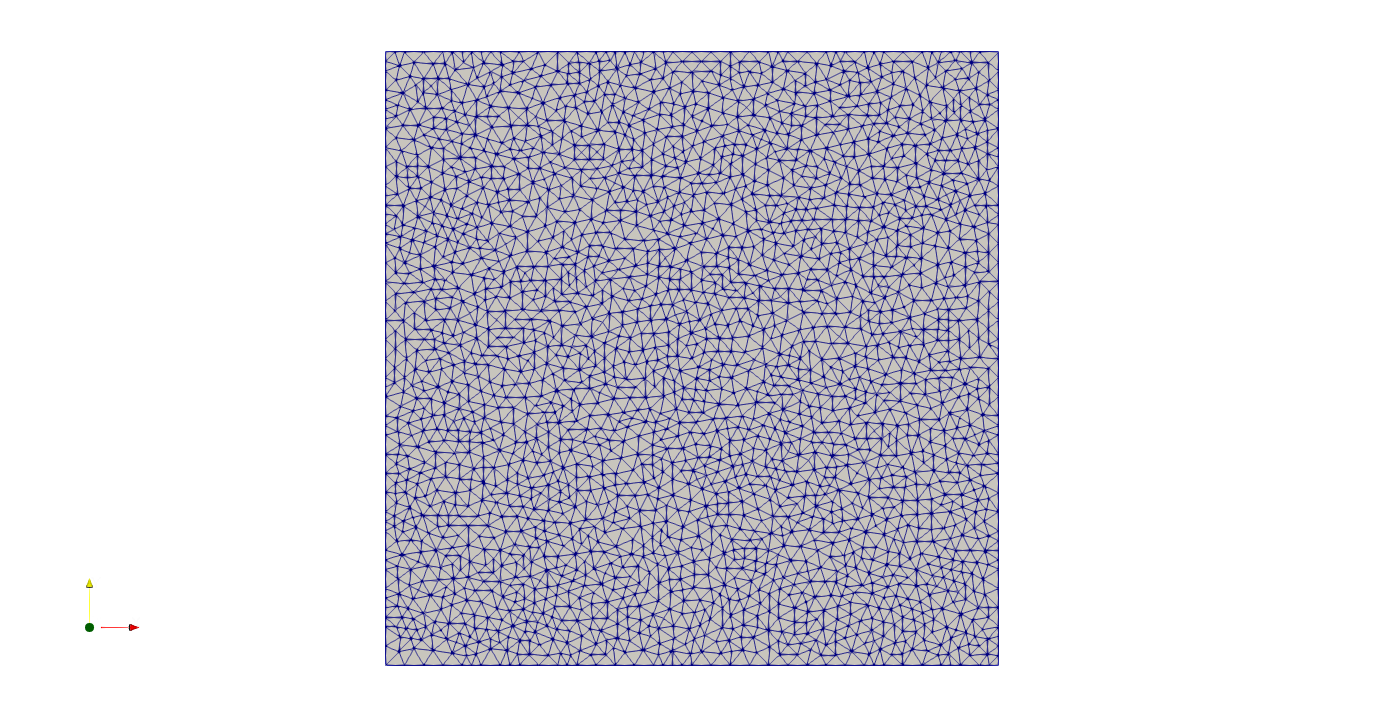
\includegraphics[width=\textwidth]{meshsquare}
    \caption{Mesh of a square with sidelength 2}
    \label{fig:meshsquare}
\end{figure}
They can be seen in figures \ref{fig:mesh} and \ref{fig:meshsquare}.
We used the unit disc for the following simulation cases:
\begin{itemize}
    \item Convergence of our implementation
    \item Startup flow (fluid at rest in the beginning but perpendicular pressure)
\end{itemize}
The square had applications in these cases:
\begin{itemize}
    \item Startup flow
    \item \enquote{ideal} rheometer cross-section
\end{itemize}
The reason why we simulated the startup flow case twice will be obvious once we compare the results. Videos of these testcases will be appended to the presentation and to the CD that accompanies this work.
\subsection{Convergence}
In this section we will use a setup to show the convergence of the implementation and the order of convergence. We will use the unit disc as our domain. We want 
\begin{equation}
u = 0\quad\forall\bfx\in\partial\Omega.
\end{equation}
We want to show the convergence for the \textsc{Maxwell} model $(\mu_s=0)$, because it is more challenging due to the missing dissipation term.
We set the initial conditions
\begin{equation}
u(t=0) = e^{-\norm{x}_2-1}-1,
\quad\bfC(t=0) = -2\bfx(e^{-(\norm{x}_2^2 -1)}-1)
\end{equation}
where $\bfx\in\Omega$ and $e$ the usual notation for the \textsc{Eulerian} number. This initial condition is obviously continuous at the boundary. Because the exact solution of this equation is not known, we will use the concept of \emph{manufactured solution}. This means that we modify our physical problem by adding a so called residual. By doing this we can artificially create a known solution. This becomes clearer by applying this technique for our problem step by step.\par 
The first step in the process of creating a manufactured solution is to set a function, which should be the exact solution. In our case, we want the solutions to remain the initial condition. We could have introduced a time dependent solution here, but it only makes calculations more complex. Next, we plug these solution functions into our equations and add the residual $\bfR\colon\Omega\to\rr^3$ on the right side. It does not matter, if we use the classic or weak formulation of our problem. By using the classic formulation we get
\begin{align}
0 &= -\partial_3 p-2\mu_p \nabla\cdot [\bfx(e^{-(\norm{x}_2^2 -1)}-1)] +\bfR_1,\\
-\frac{2}{\lambda}\bfx(e^{-(\norm{x}_2^2 -1)}-1)&= \nabla (e^{-(\norm{x}_2^2 -1)}-1) +\bfR_{2:3}.
\end{align}
Note that the time derivative evaluated to zero in both cases. Next, we solve this set of equations for $\bfR$. To do that we expand the divergence and the gradient operators to obtain
\begin{align}
\bfR_1 &= \partial_3 p +4\mu_p(e^{-(\norm{x}_2^2 -1)}(1-\norm{x}_2^2)-1),\\
\bfR_{2:3} &=2\bfx\left(e^{-(\norm{x}_2^2 -1)}\left(1-\frac{1}{\lambda}\right)+\frac{1}{\lambda}\right).
\end{align}
To solve the equations, we have to get everything back into the weak formulation. This results in 
\begin{align}
\int_\Omega(u-u^n)\psi\D\Omega +\Delta t\left(\int_\Omega\partial_3 p\psi\D\Omega + \int_\Omega\bfs\cdot\nabla\psi\D\Omega-\int_\Omega \bfR_1\psi\D\Omega\right) = 0,\\
\bfs =\mu_p\bfC_{1/\lambda},\\
\int_\Omega(\bfC_{1/\lambda} - \bfC_{1/\lambda}^n +\frac{\Delta t}{\lambda}\bfC_{1/\lambda})\cdot\varphi\D\Omega = 
\Delta t\int_\Omega \nabla u\cdot\varphi\D\Omega+\Delta t\int_{\Omega}\bfR_{2:3}\cdot\varphi\D\Omega.
\end{align}
The solution of this system is exactly our initial condition. This way we can easily calculate approximation errors. 
\begin{table}
    \centering
    \begin{tabular}{c|c|c|c|c}
        $\approx$ \# Elements per diameter& $\mathrm{L}^2$-error&EOC in $\mathrm{L}^2$&$\mathrm{L}^\infty$-error &EOC in $\mathrm{L}^\infty$\\
        \hline
        20 & 0.0797652 & - & 0.877305 & -\\
        40 & 0.0233543 & 1.77207 & 0.195846 & 2.16336\\
        80 & 0.00615334 & 1.92425 & 0.100548 & 0.96184\\
        160 & 0.00163421 & 1.91278 & 0.0369229 & 1.44529\\
        320 & 0.000433982 & 1.91288 & 0.0198643 & 0.89434
    \end{tabular}
    \caption{Convergence of the \textsc{Maxwell} model}
    \label{tab:maxwellconv}
\end{table}

Table \ref{tab:maxwellconv} shows the $\mathrm{L}^2$ error and order of convergence of this example as well as these values for the $\mathrm{L}^\infty$ norm respectively. The boundary of the domain was approximated using a polygonal chain, which increases proportionally with the number of cells. The principle of the winning least order is also applicable to the geometry. This might also explain, why in the beginning the EOC is a bit far from the expected 2. As we have 320 elements per diameter we also approximate the circle with 320 segments in the polygonal chain which, to a naked eye, is indistinguishable from a true circle. The time integration order of one is also negatively influencing the EOC. We used $\Delta t = 0.1$ and calculated until $T=1$. As the polymer viscosity we used $1$. It is typical for these kind of simulations that the $\mathrm{L}^\infty$ error is worse than $\mathrm{L}^2$. This is because it is much more sensitive for things like geometry approximations.

\subsection{Startup flow on unit disc}
We will now take a look at a more physically relevant example. Consider a fluid at rest that is subject to a perpendicular pressure gradient. This is basically the setup for the next two simulation cases. However, we will choose different domains and show that this leads to very different results. 
\begin{figure}
    \centering
    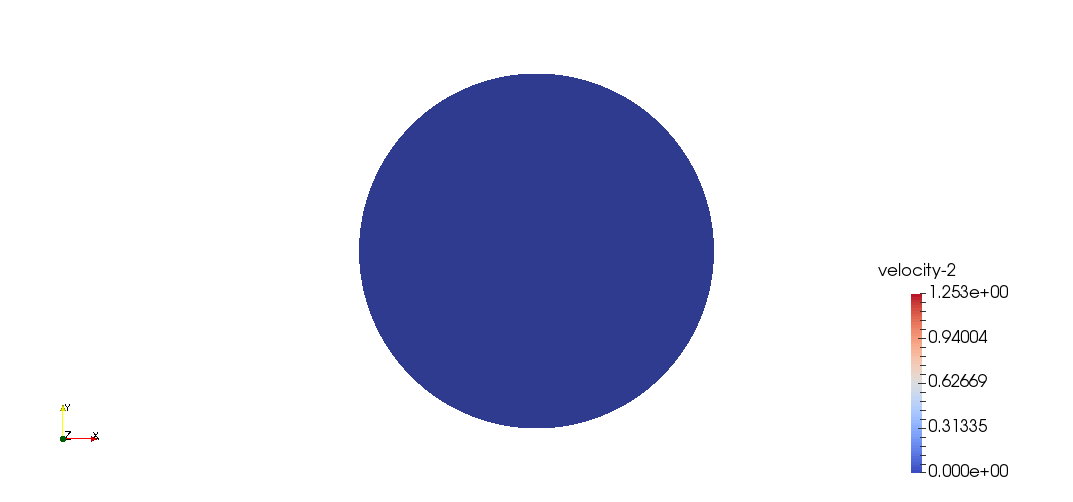
\includegraphics[width=\textwidth]{UnitDiscSetup}
    \caption{Setup startup flow unit disc}
    \label{fig:unitdiscsetup}
\end{figure}
The setup is shown in figure \ref{fig:unitdiscsetup}. We chose the no slip boundary condition $u=0$ on the boundary of the circle. We assumed a pressure gradient of $\partial_3 p=-5$ and a relaxation time of $\lambda=1$. 
\begin{figure}
    \centering
    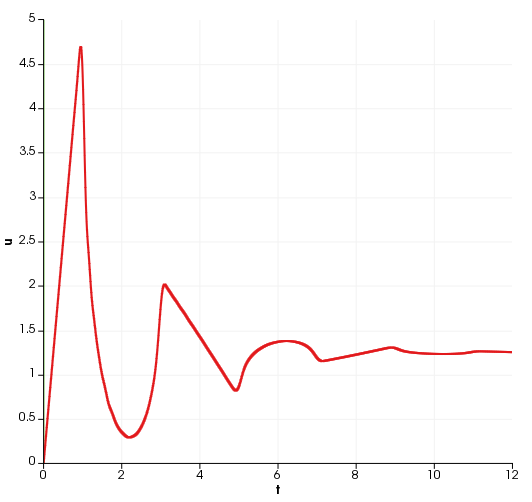
\includegraphics[width=\textwidth]{UnitDiscCenterline}
    \caption{Centerline velocity with the unit disc domain and $\mu_s=0$, $\mu_p=1$}
    \label{fig:unitdisccenterline}
\end{figure}
The centerline velocity graph is shown in figure \ref{fig:unitdisccenterline}. We used the \textsc{Maxwell} model this time with $\mu_p=1$. The typical non-\textsc{Newtonian} oscillations can be seen. We calculated until $T=12$ with $\Delta t=0.001$.
\subsection{Startup flow on square}
\begin{figure}
    \centering
    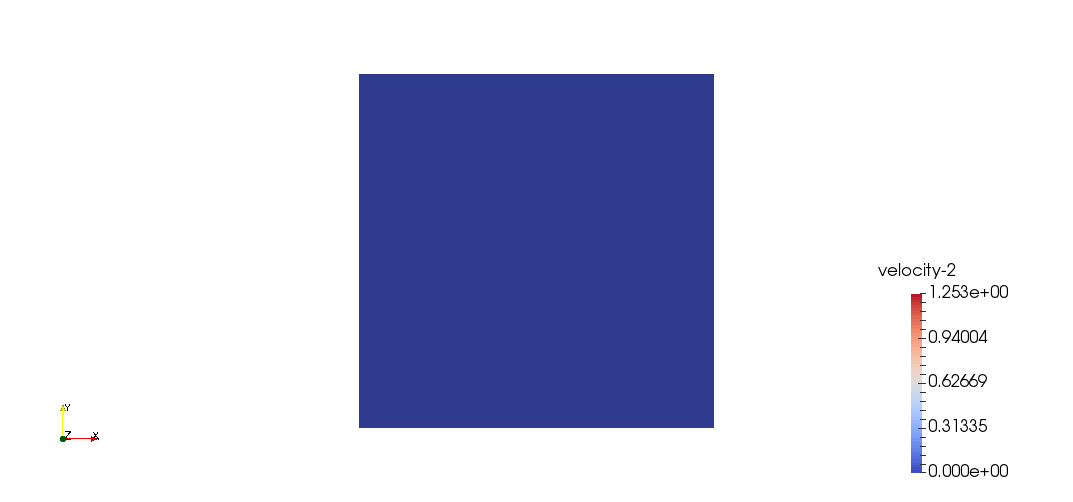
\includegraphics[width=\textwidth]{SquareSetup}
    \caption{Setup of the startup flow simulation on the square domain}
    \label{fig:squaresetup}
\end{figure}
Now we want to repeat this calculation but with a different domain. We will see that this will impact the result. The setup is shown in \ref{fig:squaresetup
}. Because we want to compare the results to \cite{A.S.RDuarte2008}, we choose periodic boundary conditions on the left and right sides and no slip boundary condition $u=0$ at the top and bottom.
\begin{figure}
    \centering
    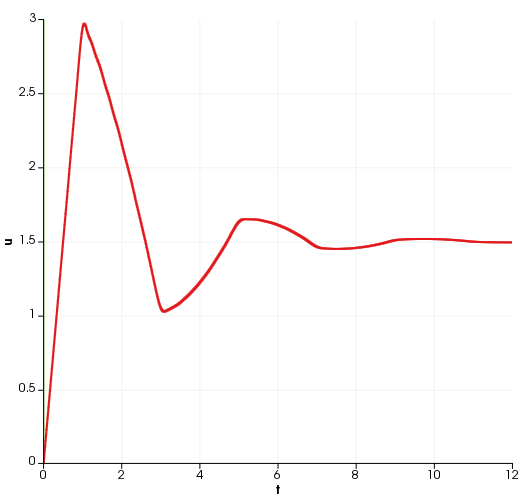
\includegraphics[width=\textwidth]{SquareCenterline}
    \caption{Centerline velocity of the start-up flow on the square domain}
    \label{fig:squarecenterline}
\end{figure}
We chose $\partial_3 p=-3$ to obtain the results from \cite{A.S.RDuarte2008} but this only effects the amplitude and not the behavior of the fluid. As one can see in figure \ref{fig:squarecenterline} we obtain a very different behavior by changing the domain.
\subsection{\enquote{Ideal} rheometer}
\begin{figure}
    \centering
    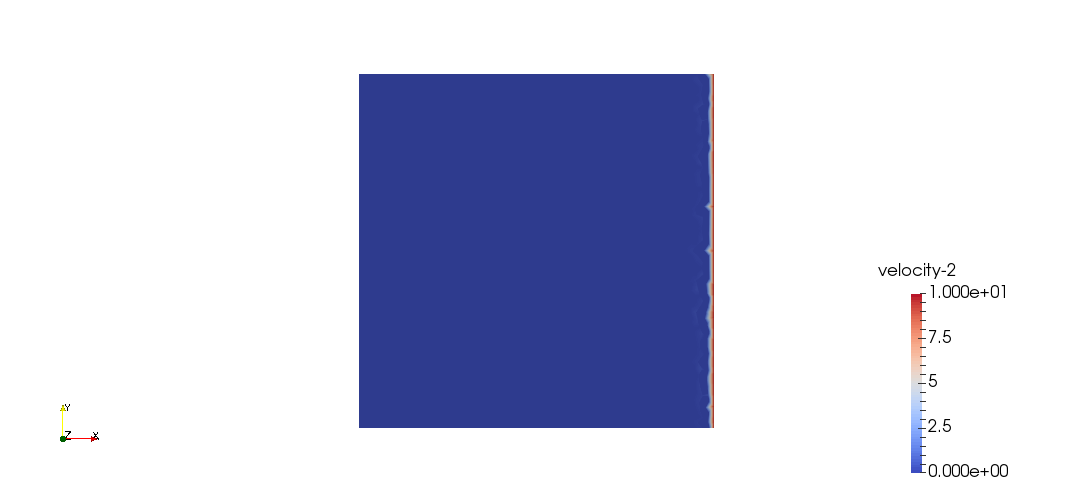
\includegraphics[width=\textwidth]{RheometerSetup}
    \caption{Setup for the rheometer simulation case}
    \label{fig:rheometersetup}
\end{figure}
The setup for this case is shown in figure \ref{fig:rheometersetup}. The left side of the square has the no slip boundary condition $u=0$. The top and bottom side are coupled with a periodic boundary condition. The right side has the \textsc{Dirichlet} boundary condition $u=10$. This case now represents a slice from top to bottom of the rheometer. However, because we assume periodic boundary conditions on the top and bottom we take the assumption of an infinitely high rheometer. 
\begin{figure}
    \centering
    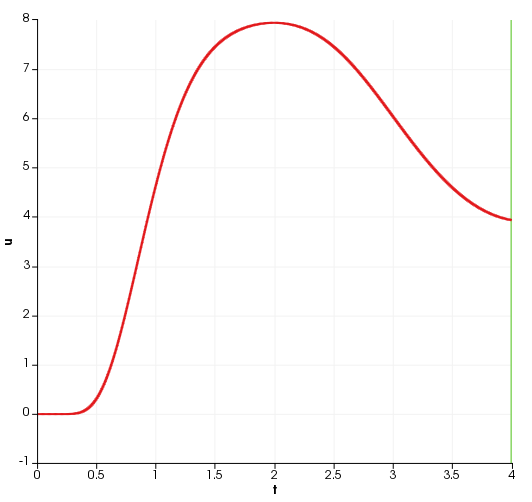
\includegraphics[width=\textwidth]{RheometerCenterline}
    \caption{Centerline velocity in the rheometer with $\mu_s=0.1$, $\mu_p=0.9$, $\lambda=2$ }
    \label{fig:rheomcenter}
\end{figure} 
\par The centerline velocity of this simulation can be seen in figure \ref{fig:rheomcenter}. We chose the \textsc{Oldroyd}-B model with $\mu_s=0.1$ and $\mu_p=0.9$. Our relaxation time was set to $\lambda=2$ and we calculated until $T=4$ with a step size of $\Delta t=0.001$. On can clearly see that we do not have a fluid that is showing \textsc{Newtonian} behavior. This would be just a monotonous function to the steady state velocity without any maximums.
\chapter{Different approaches for the integral equation}
In chapter \ref{ch:model} we could eliminate the integral from the equation completely by taking sensible assumptions on the memory function $G$. However, this is a very specific case and the more complex physical models do not have this nice feature. In this chapter we will discuss possibilities for a more general approach. 
\section{Linear combination of relaxation times}
In physics, most of the time it is sufficient to model the fluid's behavior using a linear combination of relaxation times. So let $N$ be an integer then we set
\begin{equation}
    G(\tau)=\sum_{n=1}^{N}\mu_p^{(n)}e^{-\tau/\lambda_n},
\end{equation}
where $\mu_p^{(n)}$ and $\lambda_n$ are a sets of polymer viscosities and relaxation times respectively. You can think of this process as interpolating the spectrum of the fluid's relaxation times. We will now deduce a new formula for $\bfs$ by putting in our assumption. This yields
\begin{equation}
    \bfs(t)=\int_0^t\partial_\tau \bfb(t,t-\tau)\sum_{n=1}^{N}\mu_p^{(n)}e^{-\tau/\lambda_n}\D\tau.
\end{equation}
Because all $\mu_p^{(n)}$ are constant and the integral operator is linear we can rewrite this to read
\begin{equation}
    \bfs(t) = \sum_{n=1}^{N}\mu_p^{(n)}\int_0^t\partial_\tau \bfb(t,t-\tau)e^{-\tau/\lambda_n}\D\tau.
\end{equation}
We will now follow a similar pattern as we did in chapter \ref{ch:model}. We will use integration by parts. It results
\begin{equation}
    \bfs(t)=\sum_{n=1}^{N}\left(\mu_p^{(n)}\bfb(t,0)e^{-t/\lambda_n}-\mu_p^{(n)}\bfb(t,t)+\frac{\mu_p^{(n)}}{\lambda_n}\int_0^t\bfb(t,t-\tau)e^{-\tau/\lambda_n}\D\tau \right).
\end{equation}
We can now use the initial condition on $\bfb$ to eliminate some terms. The integral can also be extended to $\infty$ without changing the value. We obtain
\begin{equation}
    \bfs(t)=\sum_{n=1}^N\frac{\mu_p^{(n)}}{\lambda_n}\int_0^\infty\bfb(t,t-\tau)e^{-\tau/\lambda_n}\D\tau.
\end{equation}
But this integral is exactly the \textsc{Laplace}-Transform of $\bfb$. So our equation for $\bfs$ becomes
\begin{equation}
    \bfs(t)=\sum_{n=1}^N\frac{\mu_p^{(n)}}{\lambda_n}L_{\bfb}(t,1/\lambda_n)=\sum_{n=1}^N\mu_p^{(n)}\bfC_{1/\lambda_n}.
\end{equation}
If we look closely at the equation above one can see that we now have $N$ equations for $\bfC$ to simulate. So to calculate $\bfs$ we have to simulate 
\begin{equation}
    \partial_t \bfC_{1/\lambda_n}+\frac{1}{\lambda_n}\bfC_{1/\lambda_n}=\nabla u
\end{equation}
for all $n$. This increases the computational effort but should still be more efficient than brute force calculating the integral at every timestep. Because $G$ is just a linear combination, all proofs and statements we made about the simpler equation remain true for this one.
\section{A simple integral equation}
In this section we will take a look at a related integral equation. This has the same complexity regarding the integral as the ones we were looking at earlier, but the complexity regarding dimension and number of equations is much reduced. This makes it easier to concentrate on the main problem and to gather ideas, how one may approach the problem in general. We use 
\begin{align}
   \dot\phi(t)&=-\phi(t)-\int_0^tm(t-\tau)\dot\phi(\tau)\D\tau,\\
   m(t)&=v_1\phi(t)+v_2\phi(t)^2,
\end{align}
where we use the dot notation for the derivative. $v_1$ and $v_2$ are given constants.
From functional analysis we can see that the integral is the convolution of $m$ and $\dot\phi$. The convolution is symmetric and the derivative can be applied to the whole product instead of just $\phi$. This is allowed, because if $\phi$ is differentiable then $m$ is as well. Using this ideas we get
\begin{equation}
    \dot\phi(t)=-\phi(t)-\int_0^t\frac{\D}{\D t}(m(\tau)\phi(t-\tau))\D\tau.
\end{equation}
If we apply the inverse Leibniz rule for parameter integrals, we can swap the integral and differential to obtain
\begin{equation}
    \dot\phi(t)=-\phi(t) -\frac{\D}{\D t}\int_0^t m(\tau)\phi(t-\tau)\D\tau +m(t)\phi(0)
\end{equation}
We can now integrate over $t$ to eliminate all differentials. This leads to 
\begin{equation}
    \phi(t)=\phi(0)-\int_0^tm(t')\phi(t-t')\D t' +\int_0^tm(t')\phi(0)\D t' -\int_0^t\phi(t')\D t',
\end{equation}
where we substituted the integration variable to $t'$ to be able to shorten the expression. We obtain
\begin{equation}
    \phi(t)=\phi(0)+\int_0^t[m(t')(\phi(0)-\phi(t-t'))-\phi(t')]\D t'.\label{eq:phianalytic}
\end{equation}
Now we have a pure integral equation. The next step will be to discretize the integral and $t$.
We will use timesteps $0=t_0,\dotsc,t_N=T$, where $T$ is the end time. The timestep length is given by $h_j=t_{j+1}-t_j$, where $h_j$ does not have to be constant. For the integral we will use 
\begin{equation}
    \int_0^{t_n}f(t)=\sum_{j=0}^{n-1}\int_{t_j}^{t_{j+1}}f(t)\D t\label{eq:generalint}
\end{equation}
for a generic $f$. Now, we have to choose a method for calculating the integral in \eqref{eq:generalint}. By using the trapezoidal rule and $h_j\equiv \Delta t$, we could solve this problem in $\mathcal{O}(N^2)$ calculations. But that is very inefficient so we will try to find a better method.
\subsection{Exponentially increasing time intervals}
We try to use the knowledge, that the resulting solution $\phi$ is exponentially declining (can be easily seen by setting $v_1=v_2=0$). Therefore it would make sense that we use intervals that increase their size exponentially. A similar trick is done in calculating the Fast-\textsc{Fourier}-Transformation. So we set $t_j=h2^j$ and choose 
\begin{equation}
    \sum_{j=0}^{n-1}\int_{t_j}^{t_{j+1}}f(t)\D t\approx\sum_{j=0}^{n-1}h_jf_{j+1}.
\end{equation}
So we approximate the integral with the rectangle formed by the value on the right side and the interval length. This underestimates the true value. Replacing the integral in \eqref{eq:phianalytic} yields
\begin{equation}
    \phi_n = \phi_0 + \sum_{j=0}^{n-1}h_j[m_{j+1}(\phi_0-\phi(t_n-t_{j+1}))-\phi_{j+1}]\label{eq:phidisc}
\end{equation} 
If we take the same equation for $\phi_{n+1}$ and subtract \eqref{eq:phidisc} we obtain
\begin{equation}
    \phi_{n+1}= \phi_n -h_n\phi_{n+1}+\sum_{j=0}^{n-1}h_jm_{j+1}(\phi(t_n-t_{j+1})-\phi(t_{n+1}-t_{j+1}))\label{eq:phidiff}
\end{equation}
But we run into a problem because of the terms $\phi(t_n-t_{j+1})$ and $\phi(t_{n+1}-t_{j+1})$. Because the difference in the argument does not necessarily correspond to a point in time we already calculated, we have to interpolate this value. To get an idea which values would make sense to use for the interpolation, we check in which interval the differences would lie in. It results
\begin{equation}
    t_n =h2^n\ge t_n-t_{j+1}=h(2^n-2^{j+1})\ge h(2^n-2^{n-1}) =h2^{n-1}=t_{n-1},
\end{equation}
where $0\le j\le n-2$. The case where $j=n-1$ is trivial and we will consider this term separately later on.
This means that the first term lies completely in the already known interval from the previous timestep. We could choose any interpolation. We use $\phi(t_n-t_{j+1})\approx\phi_n$ for all $0\le j\le n-2$ to keep it simple. If we conduct the same calculations for the second term, we get
\begin{equation}
    t_{n+1}=h2^{n+1}\ge t_{n+1}-t_{j+1}\ge h(2^{n+1}-2^{n-1})=h\frac{3}{2}2^n=\frac{3}{2}t_n,
\end{equation}
where $0\le j\le n-2$ as before. This however presents the challenge, that the interpolating lies in the yet unknown interval $[t_{n+1},3/2t_{n}]$. We hope to achieve greater accuracy by taking $t_{n+1}$. Putting the assumptions for the interpolation into \eqref{eq:phidiff} we obtain
\begin{equation}
    \phi_{n+1}(1 + h_n + \sum_{j=0}^{n-2}h_jm_{j+1})=\phi_n(1+\sum_{j=0}^{n-2}h_jm_{j+1})+h_{n-1}m_n(\phi_0-\phi_n).
\end{equation}
If we now define $s_n:=\sum_{j=0}^{n-2}h_jm_{j+1}$, we can rewrite everything as
\begin{align}
    \phi_{n+1}(1+h_n+s_n)&=\phi_n(1+s_n-h_{n-1}m_n)+h_{n-1}m_n\phi_0,\\
    s_{n+1}&=s_n+h_{n-1}m_n.
\end{align}
We define $s_0=0$ as the initial condition of $s$. To obtain greater accuracy we should eliminate the division of large numbers. Therefore we multiply the equation with $2^{-n}$. This results in
\begin{align}
    \phi_{n+1}(2^{-n}+h+2^{-n}s_n) &= \phi_n(2^{-n}+2^{-n}s_n-\frac{h}{2}m_n)+\frac{h}{2}m_n\phi_0,\\
    s_n=s_n+h_{n-1}m_n.
\end{align}
We introduce $\beta_n=2^{-n}s_n$. We obtain
\begin{align}
     \phi_{n+1}(2^{-n}+h+\beta_n) &= \phi_n(2^{-n}+\beta-\frac{h}{2}m_n)+\frac{h}{2}m_n\phi_0,\\
     \beta_{n+1} &= 2^{-n-1}s_{n+1}=\frac{1}{2}(\beta_n+\frac{h}{2}m_n) .
\end{align}
\begin{figure}
    \centering
    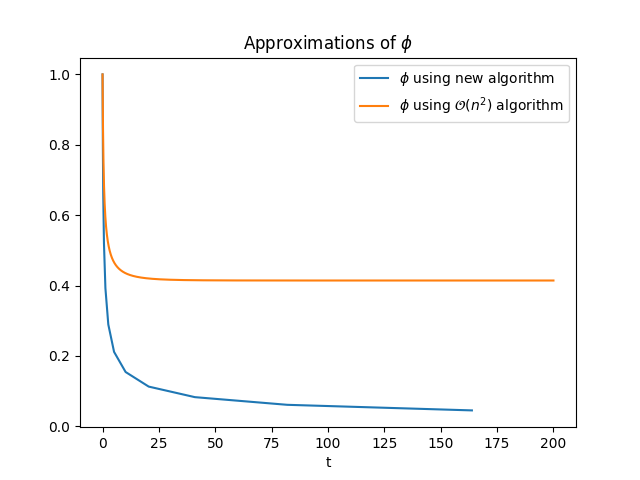
\includegraphics[width=\textwidth]{Phidiff}
    \caption{Both $\phi$ with $h=\Delta t=0.01$ and $v_1=1.5,~v_2=0.5$}
    \label{fig:phifalse}
\end{figure}
This is now an explicit algorithm with $\mathcal{O}(N)$ to solve the equation for $\phi$. However as one can see in figure \ref{fig:phifalse}, it does not converge to the correct solution. Moreover it is unclear if for $h\to 0$ the error would become better as it would lead to $h_N\to T$. This means that this method is not suitable for our problem and we need to find a new approach.
\subsection{Transformation of the argument}
The reason that the last method did not work was probably due to the fact that we eliminated the history completely. So we need an algorithm with super linear runtime. The next idea one could follow is to transform $t=f(u)$ and $\tilde\phi(u)=\phi(f(u))$, where $f$ is a diffeomorphism (bijective function with differentiable inverse).  Let $u_{-1}=f^{-1}(0)$. This is unique because $f$ is especially injective. If we recall \eqref{eq:phianalytic} and insert our transformation for $t$, we obtain
\begin{equation}
    \phi(f(u)) = \phi(f(u_{-1}))+\int_{u_{-1}}^{u}f'(u')[m(f(u'))(\phi(f(u_{-1}))-\phi(f(u)-f(u')))-\phi(f(u'))]\D u'.
\end{equation}
Now we can transform $\phi$ to $\tilde\phi$. We still have not changed the contents of the equation but just the way it is expressed. The transformed equation reads
\begin{equation}
    \tilde{\phi}(u)=\tilde{\phi}(u_{-1}) +\int_{u_{-1}}^{u}f'(u')[\tilde{m}(u')(\tilde\phi(u_{-1})-\tilde{\phi}(f^{-1}(f(u)-f(u'))))-\tilde{\phi}(u')]\D u'.\label{eq:phitilde}
\end{equation}
The goal of this transformation is that we can use equally spaced points in $u$ and $u'$ but do not have effort $\mathcal{O}(N^2)$. The term that all depends on is $\tilde\phi(f^{-1}(f(u)-f(u')))$ because this is the only time that old timesteps effect the current one. Ideally 
\begin{equation}
    F(u'):=f^{-1}(f(u)-f(u'))=u,\quad u'\in(u_{-1},u]
\end{equation}
\begin{figure}
    \centering
    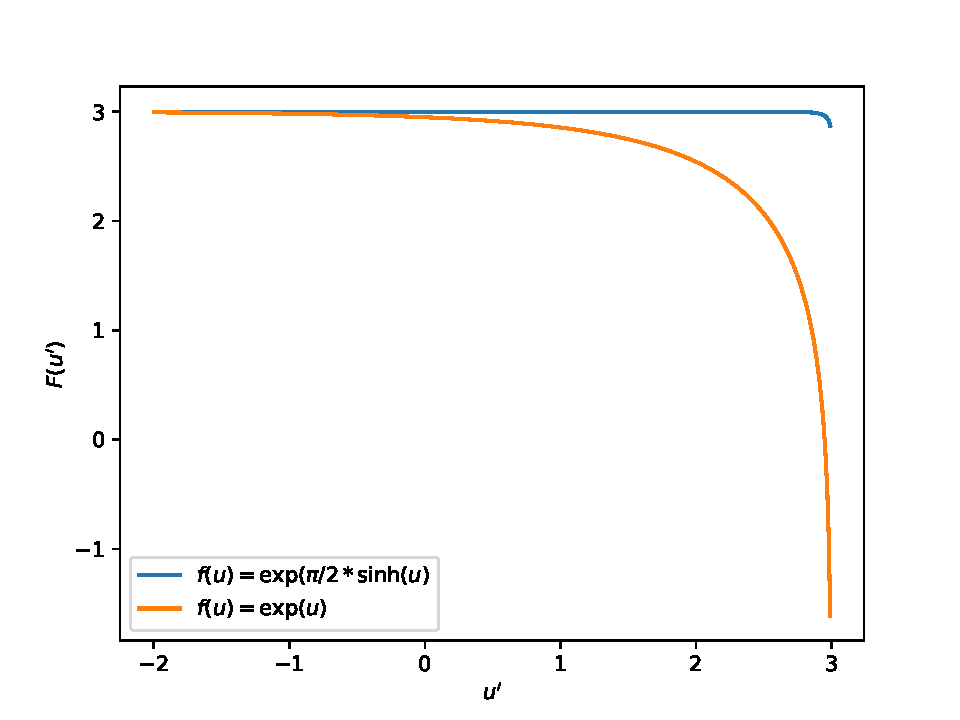
\includegraphics[width=\textwidth]{HistoryF}
    \caption{History dependency for different $f$}
    \label{fig:Fustrich}
\end{figure}
almost everywhere. This would again eliminate the history completely like in the previous example. In figure \ref{fig:Fustrich} $F(u')$ is shown for a fixed $u$. We can see that for both functions $f$ we have a long interval, in which $u=F(u')$ is a good approximation. \par 
Now let $f(u)=e^u$. We choose this because $F(u,u')$ is qualitatively the same function for every $u$ just translated. This will help us immensely later on. We then have $u_{-1}=-\infty$. Obviously we cannot start our calculation at $-\infty$ so we introduce $u_0$ where $\abs{f(u_0)-f(-\infty)}$ is negligible. From there we introduce a discretization for $u$ as
\begin{equation}
    u_i = u_0+ih,\quad\forall i=0,\dotsc,N
\end{equation}
where $h = \frac{\log(T) -u_0}{N}$ is a fixed interval length and we stop at $u_N=\log(T)$ with $T$ our end time and $N$ our given number of steps. Our goal now is to get values for all $\tilde\phi(u_i)$. We take the assumption that $\forall i=0\dotsc,N$
\begin{equation}
    \tilde\phi(u) \equiv \tilde\phi(u_i), \quad\forall u\in(u_{i-1},u_i].
\end{equation}
Let us now take a look back at \eqref{eq:phitilde} and look at the integral part by part. Let us assume we know the values for each $\tilde\phi(u_i)$ for $i\le n$ and want to calculate $\tilde\phi(u_{n+1})$. For the first part we get
\begin{equation}
    I_1:=\int_{-\infty}^{u_{n+1}}f'(u')\tilde{m}(u')\tilde\phi(-\infty)\D u'=\tilde\phi(-\infty)\sum_{i=0}^{n+1}\int_{u_{i-1}}^{u_i}f'(u')\tilde{m}(u')\D u'
\end{equation}
Now we know that $\tilde{m}$ is piecewise constant. The jump is on each integral boundary so we just get
\begin{equation}
    I_1 = \tilde{\phi}(-\infty)\sum_{i=0}^{n+1}\tilde{m}(u_i)\int_{u_{i-1}}^{u_i}f'(u')\D u' = \tilde{\phi}(-\infty)\sum_{i=0}^{n+1}\tilde{m}(u_i)[f(u_i)-f(u_{i-1})].
\end{equation}
We set 
\begin{equation}
    I_1 = \tilde\phi(-\infty)[S(n)+\tilde{m}(u_{n+1})[f(u_{n+1})-f(u_n)]].
\end{equation}
This way we can perform an update for $S(n+1) = S(n)+\tilde{m}(u_{n+1})[f(u_{n+1})-f(u_n)]$ and get only linear effort for this part. The summand for $n+1$ will have to be regarded separately because it is implicitly depending on the value of $\tilde\phi$ we are trying to calculate. We will actually discover later on that we can get a cubic problem in $\tilde\phi(u_{n+1})$ at worst which we will solve using \textsc{Newton's} method.
\par After we now handled the first part successfully we will take a look at the third part because the second will be the most challenging. Consider
\begin{equation}
    I_3:=-\int_{u_{-1}}^{u_{n+1}}f'(u')\tilde\phi(u')\D u' = -\sum_{i=0}^{n+1}\int_{u_{i-1}}^{u_i}f'(u')\tilde\phi(u')\D u'.
\end{equation} Using the same arguments as for $I_1$ we obtain
\begin{equation}
    I_3 = -\sum_{i=0}^{n+1}\tilde\phi(u_i)[f(u_i)-f(u_{i-1})] = -M(n) -\tilde\phi(u_{n+1})[f(u_{n+1})-f(u_{n})],
\end{equation}
with the update rule 
\begin{equation}
    M(n+1) = M(n) + \tilde\phi(u_{n+1})[f(u_{n+1})-f(u_{n})].
\end{equation}
For understanding the second part we will first rename the integration variable to avoid confusion
\begin{equation}
    I_2:=\int_{u_{-1}}^{u_{n+1}}f'(v)\tilde{m}(v)\tilde{\phi}(F(u_{n+1},v))\D v.
\end{equation}
Now let us recall the behavior of $F(u,v)$ in figure \ref{fig:Fustrich}. We can see that in the beginning we can set $\tilde\phi(F(u_{n+1},v))=\tilde\phi(u_{n+1})$. But what do we do with the remaining interval? To answer this question we have to see that $F$ is its own inverse in the second argument. Let $x = F(u,v)$. We want to find a $v$ for a given $u$ to solve this. We get
\begin{equation}
    f(x)=f(u)-f(v)\quad\Rightarrow f(v)=f(u)-f(x)\quad\Rightarrow v= F(u,x).
\end{equation}
The remaining discretization will be built on this fact. Specifically we set $w_i^n=F(u_n,u_i)$. This ensures that 
\begin{equation}
    \tilde\phi(F(u_{n+1},w^{n+1}_i))=\tilde{\phi}(u_j),
\end{equation}
for some $j=0,\dotsc,n$. Note that the $w_i^n$ are decreasing as $i$ increases for a fixed $n$. The lowest value of $w_i^n$ will be $w_{n-1}^n$. Our discretization $I_2$ will be 
\begin{equation}
    \{v'_i\}_i=\text{sort}(\{u_i\}_i\cup \{w_i^n\}_i),
\end{equation}
so it will differ each timestep. One might be tempted to think that this will at least result in an $\mathcal{O}(N^2)$ algorithm because we have to sort every timestep, but we will solve this issue later on.
\par An important thing to know during the simulation, is the first index $j$ so that $v'_j\in\{w_i^n\}$ for each $n$. Because we know that $v'_j = w_{n-1}^n$ we can calculate this directly. We introduce 
\begin{equation}
    l*:=\left\lceil  \frac{u_n -w_{n}^{n+1}}{h}\right\rceil.
\end{equation}
This is constant in $n$ and equals the number of intervals, which the $w_i^n$ spread. Therefore we know that all interval until $u_{n-l*+1}$ do not contain any points $w_i^{n+1}$. So we will divide the integral $I_2$ to become
\begin{equation}
    I_2 = \int_{-\infty}^{u_{n-l*+1}}f'(v)\tilde{m}(v)\tilde{\phi}(F(u_{n+1},v))\D v + \int_{u_{n-l* +1}}^{u_{n+1}}f'(v)\tilde{m}(v)\tilde{\phi}(F(u_{n+1},v))\D v.
\end{equation}
We will assume that \begin{equation}
    \tilde\phi(F(u_{n+1},v))=\tilde\phi(u_{n+1})
\end{equation}
in the first part of this integral. So we get 
\begin{equation}
    I_2 = \tilde\phi(u_{n+1})\int_{-\infty}^{u_{n-l*+1}}f'(v)\tilde{m}(v)\D v+ \int_{u_{n-l* +1}}^{u_{n+1}}f'(v)\tilde{m}(v)\tilde{\phi}(F(u_{n+1},v))\D v.
\end{equation}
By using similar argument to $I_1$ and $I_3$ we can simplify this to 
\begin{equation}
    I_2 = \tilde{\phi}(u_{n+1})\sum_{i=0}^{n+1-l*}\tilde{m}(u_i)[f(u_i)-f(u_{i-1})]+ \int_{u_{n-l* +1}}^{u_{n+1}}f'(v)\tilde{m}(v)\tilde{\phi}(F(u_{n+1},v))\D v.
\end{equation}
We will denote the remaining integral by $I_{2,2}$. Let us introduce $j*$ as the index of $w_i^{n}$ so that $w_{l*-i}^{n+1}\in[u_n,u_{n+1}],\quad\forall i\ge j*$. This can also be calculated in the preprocessing of the calculation by using the problem: Find $j*$ such that
\begin{equation}
    \frac{u_{l*}-w_{l*-j*}^{l*}}{h}\le 1 \quad \text{and} \quad\frac{u_{l*}-w_{l*-j*+1}^{l*}}{h}\g 1.
\end{equation}
This is a well-defined problem because such $j*$ always exists at timestep $l*$. We can now divide $I_{2,2}$ to obtain
\begin{equation}
    I_{2,2}= \int_{u_{n-l*+1}}^{w^{n+1}_{n+1-j*}}f'(v)\tilde{m}(v)\tilde{\phi}(F(u_{n+1},v))\D v + \int_{w^{n+1}_{n+1-j*}}^{u_{n+1}}f'(v)\tilde{m}(v)\tilde{\phi}(F(u_{n+1},v))\D v.
\end{equation}
But because the second integral lies completely within $[u_n,u_{n+1}]$ we get 
\begin{align}
    I_{2,2}&=\int_{u_{n-l*+1}}^{w^{n+1}_{n+1-j*}}f'(v)\tilde{m}(v)\tilde{\phi}(F(u_{n+1},v))\D v \\&+\tilde{m}(u_{n+1})\sum_{i=0}^{n+1-j*}\int_{w^{n+1}_{n+1-j*-i}}^{w^{n+1}_{n+1-j*-i-1}}f'(v)\tilde{\phi}(F(u_{n+1},v))\D v.
\end{align}
But be wanted that $\tilde\phi$ is constant on each interval. Therefore we want $\tilde\phi(F(u_{n+1},v))$ to be $\tilde\phi(u_{n+1-j*-i})$. We then get
\begin{align}
I_{2,2}&=\int_{u_{n-l*+1}}^{w^{n+1}_{n+1-j*}}f'(v)\tilde{m}(v)\tilde{\phi}(F(u_{n+1},v))\D v \\&+\tilde{m}(u_{n+1})\sum_{i=0}^{n+1-j*}\tilde\phi(u_{n+1-j*-i})[f(w^{n+1}_{n+1-j*-i-1})-f(w_{n+1-j*-i}^{n+1})]
\end{align}
If we recall the definition of $w$ we can simplify the expression to
\begin{align}
I_{2,2}&=\int_{u_{n-l*+1}}^{w^{n+1}_{n+1-j*}}f'(v)\tilde{m}(v)\tilde{\phi}(F(u_{n+1},v))\D v \\&+\tilde{m}(u_{n+1})\sum_{i=0}^{n+1-j*}\tilde\phi(u_{n+1-j*-i})[f(u_{n+1-j*-i})-f(u_{n+1-j*-i-1})].
\end{align}
By reordering the sum we obtain
\begin{equation}
    I_{2,2}=\int_{u_{n-l*+1}}^{w^{n+1}_{n+1-j*}}f'(v)\tilde{m}(v)\tilde{\phi}(F(u_{n+1},v))\D v +
    \tilde{m}(u_{n+1})\sum_{i=0}^{n+1-j*}\tilde\phi(u_{i})[f(u_i)-f(u_{i-1})].
\end{equation}
We can directly identify how the integral over the interval $[u_{n+1-l*},w^{n+1}_{n}]$ should be calculated. We obtain 
\begin{equation}
    \int_{u_{n-l*+1}}^{w^{n+1}_n}f'(v)\tilde{m}(v)\tilde{\phi}(F(u_{n+1},v))\D v = \tilde\phi(u_{n+1})\tilde{m}(u_{n-l*+2})[f(w^{n+1}_n)-f(u_{n-l*+1})].
\end{equation}
But it holds
\begin{equation}
    f(w^{n+1}_n)=f(u_{n+1})-f(u_n).
\end{equation}
So it yields
\begin{align}
     \int_{u_{n-l*+1}}^{w^{n+1}_n}f'(v)\tilde{m}(v)\tilde{\phi}(F(u_{n+1},v))\D v = \tilde\phi(u_{n+1})\tilde{m}(u_{n-l*+2})[f(u_{n+1})-f(u_n)-f(u_{n-l*+1})].
\end{align}
So what remains of the integral is the part, where the two discretizations overlap. We also have to discuss how we can eliminate the sorting process from the main loop as this would result in $\mathcal{O}(n^2\log(n))$ effort. We know that after calculating $l*$ time steps we have the first appearance of a $w$ which is larger than $u_0$ and therefore needs consideration. But this is independent of $n$ and can be calculated in advance as a result. The part of $w$ which overlaps is exactly the part that is not entirely in the interval $[u_n,u_{n+1}]$. So it is given by
\begin{equation}
    w^{l*}_{l*-i},\quad\forall i=1,\dotsc,j*.
\end{equation}
Because the $u_i$ are equally spaced, we know that
\begin{equation}
    u_{n+1}=u_{l*}+u_{n+1-l*}.
\end{equation}
We can therefore in the loop just add $u_{n+1-l*}$ and obtain the current position of these $w$s. For each $n$ we know that the points $u_{n+1-l*},\dotsc,u_n$ overlap. By applying the shift backwards we find that the $w$ as above overlap with 
\begin{equation}
    u_i,\quad\forall i=1,\dotsc,l^*-1.
\end{equation}
This way we can define the overlapping points 
\begin{equation}
    \tilde{u}= \bigcup\left(\bigcup_{i=1}^{l*-1}u_i\bigcup_{j=1}^{j*}w^{l*}_{l*-j}\right).
\end{equation}
We can sort these in preprocessing. If we keep the permutation array that resulted during the sorting process, we can later recall, from which discretization the point came. We introduce two new variables
\begin{equation}
    q_i:=\abs{\{u_j\colon u_j\in\tilde{u} \text{ and }u_j\le\tilde{u_i} \}},\quad
    y_i:=\abs{\{w^{l*}_j\colon w^{l*}_j\in\tilde{u} \text{ and }w^{l*}_j\le\tilde{u_i} \}}.
\end{equation}
Now we gathered all the information we need in preprocessing, we can get back to $I_{2,2}$. With the new defined variables inserted we obtain
\begin{align}
    I_{2,2}&= \sum_{i=1}^{l*+j*-1}\tilde{m}(u_{n+2-l*+q_{i-1}})\tilde{\phi}(u_{n+1-y_{i-1}})[f(u_{n+1-l*}+\tilde{u_i})-f(u_{n+1-l*}+\tilde{u}_{i-1})]\\&+\tilde{m}(u_{n+1})\sum_{i=0}^{n+1-j*}\tilde\phi(u_{i-1})[f(u_i)-f(u_{i-1})] \\&+ \tilde\phi(u_{n+1})\tilde{m}(u_{n-l*+2})[f(u_{n+1})-f(u_n)-f(u_{n-l*+1})].
\end{align}
Every term of \eqref{eq:phitilde} has been discretized. The whole discretization is obtained by calculating
\begin{equation}
    \tilde\phi(u_{n+1})=\tilde\phi(-\infty) + I_1 -I_2 +I_3.
\end{equation}
This computation yields
\begin{align}
    \tilde\phi(u_{n+1})&=\tilde\phi(-\infty) +\tilde\phi(-\infty)[S(n)+\tilde{m}(u_{n+1})[f(u_{n+1})-f(u_n)]]\label{eq:discphit1}\\&-M(n)\label{eq:discphit2} -\tilde\phi(u_{n+1})[f(u_{n+1})-f(u_{n})]  -\tilde{\phi}(u_{n+1})\sum_{i=0}^{n+1-l*}\tilde{m}(u_i)[f(u_i)-f(u_{i-1})]\\&- \tilde\phi(u_{n+1})\tilde{m}(u_{n-l*+2})[f(u_{n+1})-f(u_n)-f(u_{n-l*+1})] \\&\label{eq:discphit3}-\sum_{i=1}^{l*+j*}\tilde{m}(u_{n+2-l*+q_{i-1}})\tilde{\phi}(u_{n+1-y_{i-1}})[f(u_{n+1-l*}+\tilde{u_i})-f(u_{n+1-l*}+\tilde{u}_{i-1})]\\&\label{eq:discphit4}-\tilde{m}(u_{n+1})\sum_{i=0}^{n+1-j*}\tilde\phi(u_{i})[f(u_i)-f(u_{i-1})],
\end{align}
where we have
\begin{equation}
    S(n+1) = S(n)+\tilde{m}(u_{n+1})[f(u_{n+1})-f(u_n)]
\end{equation}
and 
\begin{equation}
    M(n+1) = M(n) + \tilde\phi(u_{n+1})[f(u_{n+1})-f(u_{n})].
\end{equation}
As initial condition we set $S(-1)=M(-1)=0$. However due to the sums in \eqref{eq:discphit2} and \eqref{eq:discphit4}, we still have quadratic effort. But this can be avoided by introducing 
\begin{equation}
    O(n):=\sum_{i=0}^{n+1-l*}\tilde{m}(u_i)[f(u_i)-f(u_{i-1})]
\end{equation}
and 
\begin{equation}
    Q(n):=\sum_{i=0}^{n+1-j*}\tilde\phi(u_{i})[f(u_i)-f(u_{i-1})]
\end{equation}
with the update rules
\begin{equation}
O(n+1) = O(n)+\tilde{m}(u_{n+2-l*})[f(u_{n+2-l*})-f(u_{n+1-l*})]
\end{equation}
and 
\begin{equation}
Q(n+1) = Q(n) + \tilde\phi(u_{n+2-j*})[f(u_{n+2-j*})-f(u_{n+1-j*})].
\end{equation}
The variables $O$ and $Q$ are well defined because $l*$ and $j*$ are at least 1. 
We set 
\begin{equation}
    O(n)= \tilde{m}(-\infty)[f(u_0+(n+2-l^*)h)-f(u_0+(n+1-l^*)h]
\end{equation}
and 
\begin{equation}
Q(n)= \tilde{\phi}(-\infty)[f(u_0+(n+2-j^*)h)-f(u_0+(n+1-j^*)h)]
\end{equation}
for $n<l^*-1$ and $n<j*-1$ respectively.
Putting $O$ and $Q$ into \eqref{eq:discphit1} to \eqref{eq:discphit4} yields
\begin{align}
    \tilde\phi(u_{n+1})&=\tilde\phi(-\infty) +\tilde\phi(-\infty)[S(n)+\tilde{m}(u_{n+1})[f(u_{n+1})-f(u_n)]]\\&-M(n) -\tilde\phi(u_{n+1})[f(u_{n+1})-f(u_{n})] -\tilde{\phi}(u_{n+1})O(n)-\tilde{m}(u_{n+1})Q(n)\\&-\tilde\phi(u_{n+1})\tilde{m}(u_{n-l*+2})[f(u_{n+1})-f(u_n)-f(u_{n-l*+1})] \\&-\sum_{i=1}^{l*+j*-1}\tilde{m}(u_{n+2-l*+q_{i-1}})\tilde{\phi}(u_{n+1-y_{i-1}})[f(u_{n+1-l*}+\tilde{u_i})-f(u_{n+1-l*}+\tilde{u}_{i-1})].
\end{align}
One can observe that $l^*=1$ is a special case because then we obtain a cubic problem in $\tilde\phi$. Otherwise the problem becomes quadratic. In the code this problem will be solved using \textsc{Newton's} method.
\chapter{Conclusion}

\addcontentsline{toc}{chapter}{List of figures}
\setcounter{lofdepth}{2}
\listoffigures
\newpage
\addcontentsline{toc}{chapter}{References}
\bibliographystyle{amsplain}
\bibliography{References}{}
\newpage
\begin{otherlanguage}{ngerman}
\chapter*{Eigenständigkeitserklärung}
Hiermit versichere ich an Eides statt, dass ich die vorliegende Arbeit selbstständig und ohne die Benutzung anderer als der angegebenen  Hilfsmittel  angefertigt  habe.  
Alle  Stellen,  die  wörtlich  oder  sinngemäß  aus  veröffentlichten  und  nicht  veröffentlichten  Schriften  entnommen  wurden,  sind  als  solche  kenntlich  gemacht.  
Die  Arbeit  ist  in  gleicher  oder  ähnlicher  Form  oder  auszugsweise  im  Rahmen  einer  anderen  Prüfung  noch  nicht  vorgelegt  worden. 
Ich  versichere,  dass  die  eingereichte    elektronische    Fassung    der    eingereichten    Druckfassung    vollständig    entspricht.
\\[\bigskipamount]
Köln, \today
\\[2\bigskipamount]
Nils Dornbusch
\end{otherlanguage}
% So it is unrealistic to fulfill this demands. To better understand $F(u')$, we will have a look at figure \ref{fig:Fustrich}. On the $y$-axis we have the value of $F(u')$ which we want to be $u$ as long as possible. The $x$-axis shows the different value of $u'$. As $u'$ approaches $u$ $F(u')$ diverges to $-\infty$ because of the logarithm. However this is not a problem for us as we just want the values to be $u$ almost everywhere. This graph clearly shows that $f(u)=\exp(\frac{\pi}{2}\sinh(u))$ is more suited for our needs as it has a steeper decrease to minus infinity. To clarify, if we would choose $f(u)=e^u$, we would have to account for the history as early as approximately $u'=0$. For the other possibility this would have to happen as late as approximately $u'=2.8$. This reduces the computational effort immensely.
%\par 
%\begin{figure}
%    \centering
%    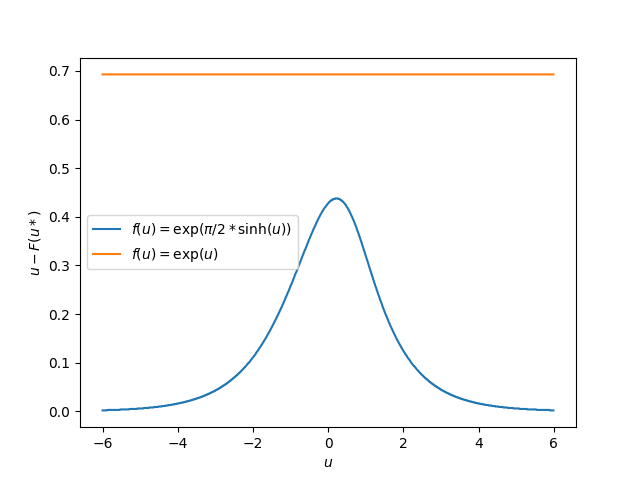
\includegraphics[width=\textwidth]{Fdiffu}
%    \caption{Minimal discretization length}
%\end{figure}
%But are these curves dependent on $u$? It could happen that $f(u)=e^u$ may be better suited for a different $u$. We will look at this behavior by calculating the intersection between $F(u')$ and the identity and plotting the y-value of this against $u$. This can be seen in figure \ref{fig:Fdiffu}. The value on the left can be interpreted as the minimal discretization length. So if we choose a cell length of less then this value we have to account for the history.  We can see that $f(u)=e^u$ is always worse. Another thing to note is that the curve for $f(u)=\exp(\frac{\pi}{2}\sinh(u))$ is not constant in $u$. That means that for every timestep we have to first check, how many parts of the approximated integral need a history part. This is what we will do next.
%\par 
%Let us recall \eqref{eq:phitilde} and insert our discretization. This leads to
%\begin{equation}
%\tilde\phi_n = \tilde\phi_0 +h\sum_{j=0}^{n-1}f'(u_{j+1})[\tilde{m}_{j+1}(\tilde\phi_0-\tilde\phi(f^{-1}(f_n-f_{j+1})))-\tilde\phi_{j+1}],
%\end{equation}
%where we used the discretization
%\begin{equation}
%\int_{u_0}^{u_n}f(u)\D u=\sum_{j=0}^{n-1}\int_{u_j}^{u_{j+1}}f(u)\D u\approx h\sum_{j=0}^{n-1}f_{j+1}.
%\end{equation}
%As one can see we can choose equally spaced points. From our previous discussion we know that we can replace $\tilde\phi(f^{-1}(f_n-f_{j+1}))$ in the intervals which lie in $[u_0,F(u*)]$. We give the last interval that lies in there the index $k(n)$. The equation then transforms to 
%\begin{align}
%\tilde\phi_n&=\tilde\phi_0+h\sum_{j=0}^{k(n)}f'(u_{j+1})[\tilde{m}_{j+1}(\tilde\phi_0-\tilde\phi_n)-\tilde\phi_{j+1}]-hf'(u_n)\tilde\phi_n\nonumber\\
%&+h\sum_{j=k(n)+1}^{n-2}f'(u_{j+1})[\tilde{m}_{j+1}(\tilde\phi_0-\tilde\phi(f^{-1}(f_n-f_{j+1})))-\tilde\phi_{j+1}]
%\end{align}
%As a next step, we want to calculate the update from $\tilde\phi_n$ to $\tilde\phi_{n+1}$. We introduce $k_{max}=\max(k(n),k(n+1))$ and $k_{min}=\min(k(n),k(n+1))$. We use $(\cdot)_{n,n+1}$ to show that depending on $k_{\max}$ and $k_{\min}$ the index can either be $n$ or $n+1$. This yields
%\begin{align}
%\tpne-\tpn&=h\sum_{j=0}^{k_{\min}}f'(u_{j+1})\tilde{m}_{j+1}(\tpn-\tpne)\\
%&+h\sum_{j=k_{\min} +1}^{k_{\max}}f'(u_{j+1})[\tilde{m}_{j+1}(\tilde\phi_0-\tilde\phi_{n,n+1})-\tilde\phi_{j+1}]\\
%&+h(f'(u_n)\tpn-f'(u_{n+1})\tpne)\\
%&+hf'(u_n)[\tilde{m}_n(\tilde\phi_0-\tilde\phi(f^{-1}(f_{n+1}-f_n)))-\tpn]\\
%&\pm h\sum_{j=k_{\min}+1}^{k_{\max}}f'(u_{j+1})[\tilde{m}_{j+1}(\tilde\phi_0-\tilde\phi(f^{-1}(f_{n,n+1}-f_{j+1})))-\tpne]\\
%&+h\sum_{j=k_{\max}+1}^{n-2}f'(u_{j+1})\tilde{m}_{j+1}(\tilde\phi(f^{-1}(f_n-f_{j+1}))-\tilde\phi(f^{-1}(f_{n+1}-f_{j+1}))).
%\end{align}
%Now, we can collect the terms, that are not part of a sum and factor out $\tpne$ and $\tpn$. We obtain
%\begin{align}
%&\tpne\left(1+h\sum_{j=0}^{k_{\min}}f'(u_{j+1})\tilde{m}_{j+1}+hf'(u_{n+1})\right)=hf'(u_n)\tilde{m}_n(\tilde\phi_0-\tilde\phi(f^{-1}(f_{n+1}-f_n)))\\
%&+\tpn\left(1+h\sum_{j=0}^{k_{\min}}f'(u_{j+1})\tilde{m}_{j+1}\right)+h\sum_{j=k_{\min}+1}^{k_{\max}}f'(u_{j+1})[\tilde{m}_{j+1}(\tilde\phi_0-\tilde\phi_{n,n+1})-\tilde\phi_{j+1}]\\
%&\pm h\sum_{j=k_{\min} +1}^{k_{\max}}f'(u_{j+1})[\tilde{m}_{j+1}(\tilde\phi(f^{-1}(f_{n,n+1}-f_{j+1})))-\tilde\phi_{j+1}]\\
%&+h\sum_{j=k_{\max}+1}^{n-2}f'(u_{j+1})\tilde{m}_{j+1}[\tilde\phi(f^{-1}(f_n-f_{j+1}))-\tilde\phi(f^{-1}(f_{n+1}-f_{j+1}))].
%\end{align}
%We see that there are two sums with the same limits. This will be dealt with now. It results
%\begin{align}
%&\tpne\left(1+h\sum_{j=0}^{k_{\min}}f'(u_{j+1})\tilde{m}_{j+1}+hf'(u_{n+1})\right)=\tpn\left(1+h\sum_{j=0}^{k_{\min}}f'(u_{j+1})\tilde{m}_{j+1}\right)\\
%&+h\sum_{j=k_{\min} +1}^{k_{\max}}f'(u_{j+1})[\tilde{m}_{j+1}(\tilde\phi_0\pm\tilde\phi_0-\tilde\phi_{n,n+1}\mp\tilde\phi(f^{-1}(f_{n,n+1}-f_{j+1})))-\tilde\phi_{j+1}\mp\tilde\phi_{j+1}]\\
%&+h\sum_{j=k_{\max}+1}^{n-2}f'(u_{j+1})\tilde{m}_{j+1}[\tilde\phi(f^{-1}(f_n-f_{j+1}))-\tilde\phi(f^{-1}(f_{n+1}-f_{j+1}))].
%\end{align}
\end{document}
